% Options for packages loaded elsewhere
\PassOptionsToPackage{unicode}{hyperref}
\PassOptionsToPackage{hyphens}{url}
\PassOptionsToPackage{dvipsnames,svgnames,x11names}{xcolor}
%
\documentclass[
  letterpaper,
  DIV=11,
  numbers=noendperiod]{scrartcl}

\usepackage{amsmath,amssymb}
\usepackage{iftex}
\ifPDFTeX
  \usepackage[T1]{fontenc}
  \usepackage[utf8]{inputenc}
  \usepackage{textcomp} % provide euro and other symbols
\else % if luatex or xetex
  \usepackage{unicode-math}
  \defaultfontfeatures{Scale=MatchLowercase}
  \defaultfontfeatures[\rmfamily]{Ligatures=TeX,Scale=1}
\fi
\usepackage{lmodern}
\ifPDFTeX\else  
    % xetex/luatex font selection
\fi
% Use upquote if available, for straight quotes in verbatim environments
\IfFileExists{upquote.sty}{\usepackage{upquote}}{}
\IfFileExists{microtype.sty}{% use microtype if available
  \usepackage[]{microtype}
  \UseMicrotypeSet[protrusion]{basicmath} % disable protrusion for tt fonts
}{}
\makeatletter
\@ifundefined{KOMAClassName}{% if non-KOMA class
  \IfFileExists{parskip.sty}{%
    \usepackage{parskip}
  }{% else
    \setlength{\parindent}{0pt}
    \setlength{\parskip}{6pt plus 2pt minus 1pt}}
}{% if KOMA class
  \KOMAoptions{parskip=half}}
\makeatother
\usepackage{xcolor}
\setlength{\emergencystretch}{3em} % prevent overfull lines
\setcounter{secnumdepth}{5}
% Make \paragraph and \subparagraph free-standing
\makeatletter
\ifx\paragraph\undefined\else
  \let\oldparagraph\paragraph
  \renewcommand{\paragraph}{
    \@ifstar
      \xxxParagraphStar
      \xxxParagraphNoStar
  }
  \newcommand{\xxxParagraphStar}[1]{\oldparagraph*{#1}\mbox{}}
  \newcommand{\xxxParagraphNoStar}[1]{\oldparagraph{#1}\mbox{}}
\fi
\ifx\subparagraph\undefined\else
  \let\oldsubparagraph\subparagraph
  \renewcommand{\subparagraph}{
    \@ifstar
      \xxxSubParagraphStar
      \xxxSubParagraphNoStar
  }
  \newcommand{\xxxSubParagraphStar}[1]{\oldsubparagraph*{#1}\mbox{}}
  \newcommand{\xxxSubParagraphNoStar}[1]{\oldsubparagraph{#1}\mbox{}}
\fi
\makeatother


\providecommand{\tightlist}{%
  \setlength{\itemsep}{0pt}\setlength{\parskip}{0pt}}\usepackage{longtable,booktabs,array}
\usepackage{calc} % for calculating minipage widths
% Correct order of tables after \paragraph or \subparagraph
\usepackage{etoolbox}
\makeatletter
\patchcmd\longtable{\par}{\if@noskipsec\mbox{}\fi\par}{}{}
\makeatother
% Allow footnotes in longtable head/foot
\IfFileExists{footnotehyper.sty}{\usepackage{footnotehyper}}{\usepackage{footnote}}
\makesavenoteenv{longtable}
\usepackage{graphicx}
\makeatletter
\newsavebox\pandoc@box
\newcommand*\pandocbounded[1]{% scales image to fit in text height/width
  \sbox\pandoc@box{#1}%
  \Gscale@div\@tempa{\textheight}{\dimexpr\ht\pandoc@box+\dp\pandoc@box\relax}%
  \Gscale@div\@tempb{\linewidth}{\wd\pandoc@box}%
  \ifdim\@tempb\p@<\@tempa\p@\let\@tempa\@tempb\fi% select the smaller of both
  \ifdim\@tempa\p@<\p@\scalebox{\@tempa}{\usebox\pandoc@box}%
  \else\usebox{\pandoc@box}%
  \fi%
}
% Set default figure placement to htbp
\def\fps@figure{htbp}
\makeatother
% definitions for citeproc citations
\NewDocumentCommand\citeproctext{}{}
\NewDocumentCommand\citeproc{mm}{%
  \begingroup\def\citeproctext{#2}\cite{#1}\endgroup}
\makeatletter
 % allow citations to break across lines
 \let\@cite@ofmt\@firstofone
 % avoid brackets around text for \cite:
 \def\@biblabel#1{}
 \def\@cite#1#2{{#1\if@tempswa , #2\fi}}
\makeatother
\newlength{\cslhangindent}
\setlength{\cslhangindent}{1.5em}
\newlength{\csllabelwidth}
\setlength{\csllabelwidth}{3em}
\newenvironment{CSLReferences}[2] % #1 hanging-indent, #2 entry-spacing
 {\begin{list}{}{%
  \setlength{\itemindent}{0pt}
  \setlength{\leftmargin}{0pt}
  \setlength{\parsep}{0pt}
  % turn on hanging indent if param 1 is 1
  \ifodd #1
   \setlength{\leftmargin}{\cslhangindent}
   \setlength{\itemindent}{-1\cslhangindent}
  \fi
  % set entry spacing
  \setlength{\itemsep}{#2\baselineskip}}}
 {\end{list}}
\usepackage{calc}
\newcommand{\CSLBlock}[1]{\hfill\break\parbox[t]{\linewidth}{\strut\ignorespaces#1\strut}}
\newcommand{\CSLLeftMargin}[1]{\parbox[t]{\csllabelwidth}{\strut#1\strut}}
\newcommand{\CSLRightInline}[1]{\parbox[t]{\linewidth - \csllabelwidth}{\strut#1\strut}}
\newcommand{\CSLIndent}[1]{\hspace{\cslhangindent}#1}

\usepackage{cancel}
\addtokomafont{disposition}{\rmfamily}
\KOMAoption{captions}{tableheading}
\makeatletter
\@ifpackageloaded{caption}{}{\usepackage{caption}}
\AtBeginDocument{%
\ifdefined\contentsname
  \renewcommand*\contentsname{Table of contents}
\else
  \newcommand\contentsname{Table of contents}
\fi
\ifdefined\listfigurename
  \renewcommand*\listfigurename{List of Figures}
\else
  \newcommand\listfigurename{List of Figures}
\fi
\ifdefined\listtablename
  \renewcommand*\listtablename{List of Tables}
\else
  \newcommand\listtablename{List of Tables}
\fi
\ifdefined\figurename
  \renewcommand*\figurename{Figure}
\else
  \newcommand\figurename{Figure}
\fi
\ifdefined\tablename
  \renewcommand*\tablename{Table}
\else
  \newcommand\tablename{Table}
\fi
}
\@ifpackageloaded{float}{}{\usepackage{float}}
\floatstyle{ruled}
\@ifundefined{c@chapter}{\newfloat{codelisting}{h}{lop}}{\newfloat{codelisting}{h}{lop}[chapter]}
\floatname{codelisting}{Listing}
\newcommand*\listoflistings{\listof{codelisting}{List of Listings}}
\usepackage{amsthm}
\theoremstyle{plain}
\newtheorem{lemma}{Lemma}[section]
\theoremstyle{plain}
\newtheorem{proposition}{Proposition}[section]
\theoremstyle{remark}
\AtBeginDocument{\renewcommand*{\proofname}{Proof}}
\newtheorem*{remark}{Remark}
\newtheorem*{solution}{Solution}
\newtheorem{refremark}{Remark}[section]
\newtheorem{refsolution}{Solution}[section]
\makeatother
\makeatletter
\makeatother
\makeatletter
\@ifpackageloaded{caption}{}{\usepackage{caption}}
\@ifpackageloaded{subcaption}{}{\usepackage{subcaption}}
\makeatother

\usepackage{bookmark}

\IfFileExists{xurl.sty}{\usepackage{xurl}}{} % add URL line breaks if available
\urlstyle{same} % disable monospaced font for URLs
\hypersetup{
  pdftitle={The behavioral effects of index insurance in fisheries},
  pdfauthor={Nathaniel Grimes; Christopher Costello; Andrew J. Plantinga},
  pdfkeywords={Index Insurance, Moral Hazard, Fisheries, Conservation},
  colorlinks=true,
  linkcolor={blue},
  filecolor={Maroon},
  citecolor={Blue},
  urlcolor={Blue},
  pdfcreator={LaTeX via pandoc}}


\title{The behavioral effects of index insurance in fisheries}
\author{Nathaniel Grimes \and Christopher Costello \and Andrew J.
Plantinga}
\date{2025-10-10}

\begin{document}
\maketitle
\begin{abstract}
Fisheries are vulnerable to environmental shocks that impact stock
health and fisher income. Index insurance is a promising financial tool
to protect fishers from environmental risk. However, insurance may
change fisher's behavior. It is imperative to understand the direction
fishers change their behavior before implementing new policies as
fisheries are vulernable to overfishing. We provide the first
theoretical application of index insurance on fisher's behavior change
to predict if index insurance will incentivize higher or lower harvests
in unregulated settings. We find that using traditional fishery models
with production variability only originating through stock abundance
implicitly leads index insurance to increase harvest. However, fishers
are adaptable and experience multiple sources of risk. Using a more
flexible specification of production shows that index insurance could
raise or lower harvest depening on the risk mitigation stragtegies
available for fishers and the design of the insurance contract. We
demonstrate the magnitude of potential change by simulating from
parameters estimated for three Norwegian fisheries. Fisheries with index
insurance contracts protecting extraction risks may increase harvest by
10\% or decrease by 2\% depending on the risk effects of inputs.
Insurance contracts protecting stock risk will always lead to harvest
increases in the range of 6-20\%. Before widespread adoption, careful
consideration must be given to how index insurance will incentivize or
disincentivize overfishing.
\end{abstract}

\renewcommand*\contentsname{Table of contents}
{
\hypersetup{linkcolor=}
\setcounter{tocdepth}{3}
\tableofcontents
}

\section{Introduction}\label{introduction}

Fisheries are exposed to numerous environmental risks that impact
biological and economic sustainability. There are limited financial
tools available to protect fishing communities against environmental
risks (Sethi 2010; Kasperski and Holland 2013). Index insurance is a new
financial tool that has significant potential to bolster community
welfare in response to disastrous weather events (Maltby \emph{et al.}
2023; Watson \emph{et al.} 2023; Hobday \emph{et al.} 2025). However,
insurance possesses moral hazards that may induce behavior change in
fishers that exacerbate overfishing. In this paper, we provide the first
examination of whether index insurance will lead to incentives that
increase or decrease fishery harvest. We apply our theoretical findings
to an empirical setting in three Norwegian fisheries.

Marine heatwaves provide a clear example of how environmental
variability impacts biological and economic productivity of fisheries.
Marine heatwaves increase animal thermal stress diminishing reproductive
ability (Barbeaux \emph{et al.} 2020), stunting growth (Pandori and
Sorte 2019), pushing species outside their usual habitats (Cavole
\emph{et al.} 2016), and may directly increase mortality (Smith \emph{et
al.} 2023). Expanding fish habitat ranges increase costs when fish move
beyond the fishing grounds of established ports (Rogers \emph{et al.}
2019). The variability from marine heatwaves impacts 77\% of species
within economic exclusion zones and reduces maximum catch potential by
6\% (Cheung \emph{et al.} 2021). Marine heatwaves are often accompanied
by harmful algal blooms and diseases leading to additional fishery
collapses (Oken \emph{et al.} 2021).

Whereas some sources of environmental variability affect fish stocks,
others affect the direct extraction of fish. Rolling seas and high wind
speeds make it more difficult to harvest (Alvarez \emph{et al.} 2006) in
addition to raising the danger to crew and vessel (Heck \emph{et al.}
2021). Storms threaten coastal infrastructure crucial to fishing
communities (Sainsbury \emph{et al.} 2019).

Fishers are highly sensitive to risk, especially income risk, and
demonstrate risk aversion despite working a seemingly risky profession
(Smith and Wilen 2005; Holland 2008; Sethi 2010). Individual choices by
fishers and fishery management mitigate environmental risk. Fishers
actively avoid fishing in destructive weather at the expense of lost
income (Pfeiffer 2020). Individual efforts to mitigate risk include
choosing consistent, known fishing grounds over risking exploring
unknown spots (Holland 2008) or choosing to fish less after storms and
hurricanes (Pfeiffer 2020; Pfeiffer \emph{et al.} 2022). However, these
efforts are unlikely to completely eliminate risk. Additional financial
tools may be needed to address income risk as a result of environmental
fluctuations (Sethi 2010; Kasperski and Holland 2013). There is growing
interest in developing new financial tools to alleviate financial and
income risk for coastal communities (Wabnitz and Blasiak 2019; Sumaila
\emph{et al.} 2020).

Insurance may be an ideal financial tool for risk management in
fisheries as it is scalable, protects against environmental shocks, and
smooths income for fishers (Mumford \emph{et al.} 2009; Watson \emph{et
al.} 2023). Currently, insurance in fisheries is primarily used to
protect assets such as vessel hulls or fishing gear (FAO 2022).
Insurance coverage could be expanded to include income variability
originating from weather and biological productivity shocks. An
insurance product covering these environmental risks could improve
fisher welfare and promote community resilience (Maltby \emph{et al.}
2023).

Policy makers have begun advocating for new fisheries insurance programs
modeled after agricultural crop insurance programs (Murkowski 2022).
Index insurance is one such product extolled by practitioners as a prime
candidate for fisheries productivity insurance (Hobday \emph{et al.}
2025). Index insurance gained traction in agriculture as an effective
alternative to indemnity crop insurance in developing countries because
it had lower administrative cost, minimizes moral hazards, and does not
require claim verification (Collier \emph{et al.} 2009; Carter \emph{et
al.} 2017). Whereas indemnity insurance requires an assessment of loss
to an individual, index insurance uses an independent measure as the
basis for issuing payouts to all policyholders. The anticipated
difficulty in establishing individual indemnified loss for individual
fishers is a key reason for the rise of index insurance in prominence
over indemnity insurance (Herrmann \emph{et al.} 2004; Watson \emph{et
al.} 2023).

An example pilot program through the Caribbean Oceans and Aqauculture
Sustainability Facility (COAST) pays out a set amount to fishers when
indices of wave height, wind speed, and storm surge indicate a hurricane
(Sainsbury \emph{et al.} 2019). Triggers are the index values that
initiate a payout. Offering new insurance programs in diverse fisheries
will require identifying additional indices and triggers to protect
against different environmental risks.

One crucial area that remains under studied is the potential influence
of insurance on fishers behavior. Moral hazards are decisions by insured
agents that they would not otherwise take if they were uninsured (Wu
\emph{et al.} 2020). Although practitioners appear to favor index
insurance on the belief that it avoids moral hazard (RARE 2021), there
are two components to insurance moral hazard: ``chasing the trigger''
and ``risk reduction'' that must be considered. ``Chasing the trigger''
is the directed behavior of policyholders to increase the likelihood of
a payout. For example, a fisher might choose to fish less to receive an
indemnified harvest insurance payment. Index insurance completely
eliminates this moral hazard if the index is independent of fisher
choices, e.g.~fishers cannot affect sea surface temperature. ``Risk
reduction'' occurs when policyholders possess an insurance contract that
protects them from risk, leading them to reoptimize their decisions.
Index insurance remains susceptible to this element of moral hazard. One
possible response by fishers is to take on additional risk by fishing
more. Alternatively, the risk protection offered by insurance could
encourage fishers to fish less as insurance payouts sufficiently cover
income loss. All preliminary analyses of fisheries index insurance are
missing rigorous assessment of risk reduction moral hazards.

In this paper, we assess how index insurance moral hazards could change
fisher input choices. Subsequently, the changes in inputs lead to
changes in harvest and thus sustainability. Fisheries remain vulnerable
to overfishing (FAO 2020). It is imperative to ensure new policies, such
as index insurance, do not provide perverse incentives that degrade long
term sustainability by encouraging greater fishing pressures.

Previous studies articulated hypothetical examples of moral hazards in
potential fishery indemnity insurance programs, such as encouraging
fishers to fish in foul weather or to not exit the fishery after a bad
year of harvest (Herrmann \emph{et al.} 2004; Watson \emph{et al.}
2023). However, neither study built testable models to uncover risk
reduction moral hazard impacts on fisheries.

Research from agriculture provides compelling evidence that behavior
change ought to be expected in fisheries. Index insurance applied to
grazing in pasture commons shows clear evidence of risk reduction moral
hazards leading to environmental degradation (Müller \emph{et al.} 2011;
Bulte and Haagsma 2021). Other studies from agriculture find that the
impact of insurance on environmental sustainability depends on the
underlying risk reducing or increasing qualities of inputs used in
production (Ramaswami 1993; Mahul 2001; Mishra \emph{et al.} 2005). Risk
increasing (decreasing) inputs will always lead to increased (decreased)
input use with insurance. Numerous agricultural studies confirm
insurance incentivizes changes in input use (Horowitz and Lichtenberg
1993; Babcock and Hennessy 1996; Smith and Goodwin 1996; Goodwin
\emph{et al.} 2004; Mishra \emph{et al.} 2005; Cai 2016; Deryugina and
Konar 2017; Claassen \emph{et al.} 2017; Elabed and Carter 2018; Sibiko
and Qaim 2020; Stoeffler \emph{et al.} 2022; Sloggy \emph{et al.} 2025).

Fisheries differ from agriculture in crucial ways, thus motivating an
analysis of the behavioral effects of index insurance in this new
setting. In a standard fisheries model, production by a fisher depends
on the abundance of the resource, as measured by the fish stock. In this
case, there is a positive relationship between output and inputs of
labor and capital. For example, more fishing boats results in a greater
catch for a given fish stock. When the fish stock is subject to
stochastic shocks, as in the marine heatwave example discussed above,
inputs will be risk-increasing and, thus, index insurance covering
biological stock risk will always increase input use and harvest of the
resource. This suggests that index insurance will be in conflict with
conservation goals in fisheries. However, fishers also face risk that is
independent of biological risk. For example, weather and wave conditions
may make it difficult to catch fish or new regulations may limit where
fishing can take place. Inputs that interact with extraction shocks may
be risk-increasing or risk-decreasing. Therefore, index insurance
applied to extraction risk has the potential to reduce harvest and
conserve fish stocks. A complete analysis of index insurance in
fisheries is needed to understand the different types of risk faced by
fishers, alternative ways in which insurance contracts can be designed,
and whether insurance will be compatible with conservation goals.

To estimate the magnitude of potential harvest changes, we numerically
simulate a model from parameter estimations of Norwegian fisheries from
Asche \emph{et al.} (2020). The Norwegian fisheries show index insurance
could raise harvest by 20\% or lower harvest by 2\% contingent on the
fishery input characteristics and contract type. All contracts specified
to protect biological stock risk showed large increases in harvest
regardless of the risk effects. Currently, most proposed insurance
contracts are examining triggers based on stock risk, such as sea
surface temperature or chlorophyll-a (Watson \emph{et al.} 2023).
Without additional constraints, these types of contracts will
incentivize greater exploitation of vulnerable fish stocks.

The remainder of the paper is structured as follows.
Section~\ref{sec-jp} demonstrates how assuming standard fishery
production models will always bias index insurance towards overfishing.
We then present a new stochastic production function for fisheries that
integrates both stock and extraction risk. Section~\ref{sec-common}
proves that index insurance will change fisher behavior, but the outcome
depends on the risk effects of inputs and the type of insurance
contract. Section~\ref{sec-multi} extends the theoretical model to
account for multiple inputs in fishing that reflects the decisions of
fishers in the empirical setting. Section~\ref{sec-sim} numerically
estimates potential harvest changes with an index insurance program.
Parameters are calibrated with an application to Norwegian fisheries
through the results of Asche \emph{et al.} (2020).
Section~\ref{sec-disc} concludes with a discussion on the suitability of
fishery index insurance.

\section{Risky Production in Fisheries}\label{sec-jp}

Here we develop a model of fishery production under risk. We are
primarily interested in within-season input decisions and risk, so we
omit time subscripts, but will be explicit about when random variables
are known, or unknown, to fishers. We begin with a canonical model of
fishery production, and then extend it to accommodate more realistic
dimensions of risk.

Fishers choose an input \(x\) that interact through an increasing
concave production technology \(f(x)\)\footnote{Common specifications of
  \(f(x)\) are Cobb-Douglas or linear harvest from Gordon-Schaefer.}.
Fish biomass is \(B\), and total production, or ``harvest'', \(y\) is
given by:

\begin{equation}\phantomsection\label{eq-trad}{
y = Bf(x)
}\end{equation}

We assume that \(B\) is unknown prior to the choice of \(x\), but that
some information on \(B\) is available. Specifically, we assume
\(B=\hat{B}+\theta\), where \(\hat{B}\) is known and \(\theta\) is mean
zero additive error term, with known variance \(\sigma^2_\theta\); we
will refer to \(\theta\) as the ``stock risk''. This implies that
equation 1 can be rewritten:

\begin{equation}\phantomsection\label{eq-trad2}{
    y = \hat{B}f(x) + \theta f(x)
}\end{equation}

This approach combines a standard model of fishery production
(Equation~\ref{eq-trad}) with the simple observation that biomass, which
affects payoffs, is unknown prior to the choice of inputs. With this
model, we can examine how index insurance affects incentives around
input choice. Under standard assumptions, fishers are price takers,
incur convex costs, and are risk averse over profits. While more general
than fisheries, Mahul (2001) studies that problem and shows that index
insurance will always lead to an increase in input use.\footnote{We
  verify Mahul's result in our formal setup in Section~\ref{sec-common}.}
In our setting, this implies that under the standard fishery production
model of Equation~\ref{eq-trad2}, index insurance will always increase
harvest.

This result immediately challenges the long term sustainability of index
insurance in fisheries. However, fishers are exposed to many margins of
risk. Anecdotally and empirically, fishers make informed decisions to
mitigate risk beyond just exposure to stock risk (Kirkley and Strand
1998; Eggert and Tveteras 2004; Kompas \emph{et al.} 2004; Smith and
Wilen 2005; Holland 2008; Sethi 2010; Pfeiffer 2020; Pfeiffer \emph{et
al.} 2022). Stock risk \(\theta\) remain an inevitable source of risk
that we must maintain in any fishery model, but we expand the standard
fishery model in Equation~\ref{eq-trad2} to Equation~\ref{eq-jpfish} by
adding a second source of risk called extraction risk, \(\omega\), and
new means of input risk reduction, \(h(x)\) to allow fishers more
margins to adjust risk exposure.

\begin{equation}\phantomsection\label{eq-jpfish}{
y=f(x)\hat{B}+\theta f(x)+\omega h(x)
}\end{equation}

All other forms of risk not captured by stock risk are extraction risk,
\(\omega\), where \(\omega\) is a random variable with
\(\mathbb{E}[\omega]=0\) and variance \(\sigma_\omega^2\). Foul weather,
regulatory changes, or inherent variability in extraction all impact
fisher production. Fisher inputs may interact with these risks through
the extraction risk effect function \(h(x)\). Extraction risk effects
may reduce or increase risk. Inputs that increase variance are called
risk increasing, \(h_x(x)>0\), and inputs that decrease variance are
called risk decreasing, \(h_x(x)<0\) (Just and Pope 1978).

We will refer to production in the form of Equation~\ref{eq-jpfish} as
``risky production''. Risky production is more flexible than the
standard fishery production model in Equation~\ref{eq-trad2} as it
allows for two sources of risk and multiple avenues for fishers to
mitigate risk. Risky production nests the standard fishery production
model as a special case when \(\omega=0\) or \(h(x)=0\). It also
maintains increasing mean production in inputs so that changes in inputs
correspond to changes in expected harvest and conservation.

With two sources of risk and adaptive margins, we have created a more
accurate representation of risky production in fisheries, but deviate
from the proven framework of Mahul (2001). Therefore, it is not
immediately clear how index insurance will affect fisher harvest
decisions with Equation~\ref{eq-jpfish}. In the the next section we
prove under what conditions insurance offered to fisheries with a
production function with the form of Equation~\ref{eq-jpfish} will
change fisher behavior and in which direction.

\section{Index insurance in fisheries}\label{sec-common}

We assume fishers derive utility from profits and are price takers. If
we set harvest from Equation~\ref{eq-jpfish} as the numeraire good so
its price is exactly equal to 1, we can define a fisher's profit
function:

\begin{equation}\phantomsection\label{eq-pi1}{
\begin{aligned}
\pi=f(x)\hat{B}+\theta f(x)+\omega h(x)-c(x)
\end{aligned}
}\end{equation}

We assess the potential behavior implications of an insurance contract
to protect against stock, \(\theta\), or extraction risk, \(\omega\). We
assume insurance companies have perfect information on both
distributions, although in reality, insurance agents may only have
sufficient information on one of the risks to form a suitable contract.
For example, stock shocks may be easier to observe and monitor compared
to individual extraction shocks.

We create insurance lotteries through contracts that use either
\(\omega\) or \(\theta\) as the trigger. For notational ease, we present
the model with a contract built on \(\omega\), but the structure is
interchangeable with contracts built on \(\theta\). Insurance pays out a
constant amount \(\gamma\) if \(\omega<\bar \omega\). By allowing
contracts on only one of the random variables, we introduce basis risk
as a contract triggered solely on \(\omega\) cannot protect against all
the biological risk of \(\theta\). We assume that \(\theta\) and
\(\omega\) are independent\footnote{In the appendix we include proofs
  when shocks are perfectly correlated, but the results become difficult
  to extract clear insights}. An example of how shocks could be
independent is that stock shocks operate at different time scales than
extraction shocks (Alvarez \emph{et al.} 2006).

Actuarially fair insurance implies the premium, \(\rho\), paid in both
lottery outcomes to be the probability of receiving a payout times the
payout amount, \(\rho=J(\bar \omega)\gamma\), where \(J(\omega)\) is the
cumulative distribution of the representative shock. Additionally, if we
set the trigger in either contract to zero, profits will enter
corresponding bad and good states when \(\omega\) is positive and
negative respectively.

Fishers are expected utility maximizers. To do so, they need to make
decisions on the marginal profitability in the good and bad states. We
introduce the following two lemmas to help us understand how marginal
profit in both states is affected by input risk effects for each type of
contract:

\begin{lemma}[]\protect\hypertarget{lem-mp}{}\label{lem-mp}

Expected marginal profit is higher in bad states for risk decreasing
inputs when contracts are built on extraction risk \(\omega\).

\(\frac{\mathbb{E}[\partial \pi|\omega<\bar \omega]}{\partial x}-\frac{\mathbb{E}[\partial \pi|\omega>\bar \omega]}{\partial x}>0\)
if \(h_{x}(x)<0\).

Otherwise, risk increasing inputs lead to higher expected marginal
profit in the good states.

\(\frac{\mathbb{E}[\partial \pi|\omega<\bar \omega]}{\partial x}-\frac{\mathbb{E}[\partial \pi|\omega>\bar \omega]}{\partial x}<0\)
if \(h_{x}(x)>0\)

\end{lemma}

\begin{lemma}[]\protect\hypertarget{lem-theta}{}\label{lem-theta}

Contracts built on \(\theta\) will always lead to higher expected
marginal profits in the good state regardless of extraction risk effects

\(\frac{\mathbb{E}[\partial \pi|\theta<\bar \theta]}{\partial x}-\frac{\mathbb{E}[\partial \pi|\theta>\bar \theta]}{\partial x}<0\)

\end{lemma}

The proofs of Lemma~\ref{lem-mp} and Lemma~\ref{lem-theta} are included
in the appendix.

Risk aversion is a necessary condition for insurance to be desirable
(Outreville 2014). Therefore, we assume fishers are risk averse to
income shocks through a concave utility function. Fishers will maximize
their own expected utility across lotteries by selecting inputs with an
exogenous insurance contract (Equation~\ref{eq-max}). Fishers consider
the joint distribution \(j(\omega,\theta)\) of shocks to maximize their
utility.

\begin{equation}\phantomsection\label{eq-max}{
\begin{aligned}
U\equiv\max_{x}\mathbb{E}[U]=\int^{\infty}_{-\infty}&\left[ \int^{\bar \omega}_{-\infty}j(\omega,\theta)u(\pi(x,\hat{B},\theta,\omega)+(1-J(\bar \omega))\gamma)d\omega \right.\\
&\left.+\int^{\infty}_{\bar{\omega}}j(\omega,\theta) u(\pi(x,\hat{B},
\theta,\omega)-J(\bar \omega)\gamma)d \omega\right] d\theta
\end{aligned}
}\end{equation}

The first order condition that solves Equation~\ref{eq-max} is then:

\begin{equation}\phantomsection\label{eq-foc1}{
\begin{aligned}
\frac{\partial U}{\partial x}=&\int^{\infty}_{-\infty}\left[ \int^{\bar \omega}_{-\infty}j(\omega,\theta)u_{x}(\pi(x,\hat{B},\theta,\omega)+(1-J(\bar \omega))\gamma)\frac{\partial \pi}{\partial x}(x,\hat{B},\theta,\omega)d\omega\right.\\
&\left.+\int^{\infty}_{\bar{\omega}}j(\omega,\theta) u_{x}(\pi(x,\hat{B},\theta,\omega)-J(\bar \omega)\gamma)\frac{\partial \pi}{\partial x}(x,\hat{B},\theta,\omega)d\omega\right] d\theta\\
&=0
\end{aligned}
}\end{equation}

To find the effect of insurance on optimal input, we use the implicit
function theorem to examine how input choice varies with the insurance
payout \(\gamma\):

\begin{equation}\phantomsection\label{eq-ivt}{
\frac{\partial x^{*}}{\partial \gamma}=-\frac{\frac{\partial U}{\partial x \partial \gamma}}{\frac{\partial^2 U}{\partial x^{2}}}
}\end{equation}

We use \(\gamma\) to test insurance effects, because a marginal change
in the payout increases the value of insurance\footnote{As shown in
  Section~\ref{sec-sim}, marginal utility reaches a maximum value before
  decreasing at high \(\gamma\). Therefore we assume the change in
  \(\gamma\) occurs at values less than the optimal insurance coverage.}.
Receiving more compensation in the bad states provides greater boosts to
utility for risk averse fishers.

By the sufficient condition of a maximization problem,
\(\frac{\partial^2 U}{\partial x^{2}}\) is negative so we can focus
solely on the numerator to sign the effect. The numerator of
Equation~\ref{eq-ivt} is given by:

\begin{equation}\phantomsection\label{eq-xgam}{
\begin{aligned}
\frac{\partial U}{\partial x \partial \gamma}=\int^{\infty}_{-\infty}\left[ \int^{\bar \omega}_{-\infty}j(\omega,\theta)u''(\pi(x,\hat{B},\theta,\omega)+(1-J(\bar \omega))\gamma)\frac{\partial \pi}{\partial x}(x,\hat{B},\theta,\omega)(1-J(\bar \omega))d\omega\right.\\
+\left.\int^{\infty}_{\bar{\omega}}j(\omega,\theta) u''(\pi(x,\hat{B},\theta,\omega)-J(\bar \omega)\gamma)\frac{\partial \pi}{\partial x}(x,\hat{B},\theta,\omega)(-J(\bar \omega))d\omega\right] d\theta
\end{aligned}
}\end{equation}

We examine the input decisions of insurance contingent on the source of
risk the insurance is designed to protect. Proposition~\ref{prp-ind}
demonstrates that contracts built on extraction risks depend on the
underlying input risk effects.

\begin{proposition}[]\protect\hypertarget{prp-ind}{}\label{prp-ind}

For feasible index insurance contracts specified at trigger
\(\bar\omega=0\), optimal fisher harvest will decrease with an increase
in \(\gamma\) when \(h_x(x)<0\) and increase when \(h_x(x)>0\).

\end{proposition}

\begin{proof}
Independence of \(\omega\) and \(\theta\) allows us to factor out the
joint distribution in the integral of Equation~\ref{eq-xgam} into the
respective marginal distributions shown by \(j_\theta(\theta)\) and
\(j_\omega(\omega)\) respectively.

\begin{equation}\phantomsection\label{eq-egam}{
\begin{aligned}
\frac{U}{\partial x \partial \gamma}=\int^{\infty}_{-\infty}j_{\theta}(\theta)\left[ \int^{\bar\omega}_{-\infty}j_{\omega}(\omega)u''(\pi(x,\hat{B},\theta,\omega)+(1-J(\bar\omega))\gamma)\frac{\partial \pi}{\partial x}(x,\hat{B},\theta,\omega)(1-J(\bar\omega))d\omega\right.\\
+\left.\int^{\infty}_{\bar{\omega}}j_{\omega}(\omega) u''(\pi(x,\hat{B},\theta,\omega)-J(\bar\omega)\gamma)\frac{\partial \pi}{\partial x}(x,\hat{B},\theta,\omega)(-J(\bar\omega))d\omega\right] d\theta
\end{aligned}
}\end{equation}

Suppose insurance fully covers the loss between states, then utility in
the good state and bad state are equal to each other so that we can
factor out like terms in Equation~\ref{eq-egam}. For brevity, all like
terms including \(\gamma\) are indicated by \(u(\cdot)\).

\begin{equation}\phantomsection\label{eq-simp}{
\begin{aligned}
\frac{U}{\partial x \partial \gamma}=\int^{\infty}_{-\infty}&j_{\theta}(\theta)J(\bar\omega)(1-J(\bar\omega))u''(\theta,\cdot)\\
&\times\left[ \int^{\bar\omega}_{-\infty}j_{\omega}(\omega)\frac{\partial \pi}{\partial x}(x,\hat{B},\theta,\omega)d\omega
-\int^{\infty}_{\bar{\omega}}j_{\omega}(\omega)\frac{\partial \pi}{\partial x}(x,\hat{B},\theta,\omega)d\omega\right] d\theta
\end{aligned}
}\end{equation}

The first term outside the brackets is negative by the definition of
concave utility, \(u''<0\). Lemma~\ref{lem-mp} demonstrates the interior
of the brackets is positive when \(h_x(x)<0\) as the marginal profit in
the bad state is greater than the marginal profit in the good.
Therefore, index insurance will decrease input use for risk decreasing
inputs when the extraction shocks are independent of stock shocks.

When \(h_x(x)>0\), the interior sign of the brackets in
Equation~\ref{eq-simp} is negative by Lemma~\ref{lem-mp}. Therefore,
index insurance will increase input use for risk increasing inputs.

Direction of input change will exactly match the direction of harvest
change by the poroperties of the production function.
\end{proof}

Proposition~\ref{prp-ind} shows contracts specified on extraction risk
could have positive or negative effects on conservation depending on the
risk effects of the input. Insurance lowers the use of risk decreasing
inputs because the need to protect against risk with that input is
replaced by the risk mitigating qualities of insurance. Insurance
increases risk increasing inputs as it protects against additional risk
allowing fishers to expand production without taking on greater risk.
The stock effect persists when contracts are specified on extraction
risks, but are not influential in the decision. Instead, if we specify a
contract on the stock shocks, then the stock risk effects become more
prevalent and distinctly changes the harvest outcome.

\begin{proposition}[]\protect\hypertarget{prp-theta}{}\label{prp-theta}

For feasible index insurance contracts specified at trigger
\(\bar\theta=0\), optimal harvest will always increase with an increase
in \(\gamma\).

\end{proposition}

\begin{proof}
A contract built with \(\theta\) will follow the same steps as the proof
for Proposition~\ref{prp-ind} with the only difference being in the
integral bounds and the differential variables as shown in
Equation~\ref{eq-gstheta}. The 2nd term of Equation~\ref{eq-gstheta} is
always negative by Lemma~\ref{lem-theta}. Therefore, a contract built on
\(\theta\) will always increase optimal input use.

\begin{equation}\phantomsection\label{eq-gstheta}{
\begin{aligned}
\frac{U}{\partial x \partial \gamma}=\int^{\infty}_{-\infty}&j_{\omega}(\omega)J(\bar\theta)(1-J(\bar\theta))u''(\omega,\cdot)\\
&\times\left[ \int^{\bar\theta}_{-\infty}j_{\theta}(\theta)\frac{\partial \pi}{\partial x}(x,\hat{B},\theta,\omega)d\theta
-\int^{\infty}_{\bar{\theta}}j_{\theta}(\theta)\frac{\partial \pi}{\partial x}(x,\hat{B},\theta,\omega)d\theta\right] d\omega
\end{aligned}
}\end{equation}

The change in input use will lead to higher expected optimal harvest.
\end{proof}

Proposition~\ref{prp-theta} demonstrates a clear bias towards
overfishing with contracts solely specified on \(\theta\). Increased
stock abundance directly leads to higher variance. Insurance protects
against the additional risk and encourages fishers to expand production.

The same intuition explains why the standard fishery production model
implicitly leads to overfishing with index insurance. We can simplify
our model framework to stock risk as the only random variable to match
the standard fishery production model in Equation~\ref{eq-trad2}. Then
we can verify Mahul (2001) result for standard fishery production.

\begin{proposition}[]\protect\hypertarget{prp-std}{}\label{prp-std}

For feasible insurance contracts specified at trigger \(\bar\theta=0\)
with production function \(y=Bf(x)+\theta f(x)\), optimal harvest will
always increase with an increase in \(\gamma\).

\end{proposition}

\begin{proof}
With one random variable, Equation~\ref{eq-gstheta} simplifies to
Equation~\ref{eq-ps}:

\begin{equation}\phantomsection\label{eq-ps}{
\begin{aligned}
\frac{U}{\partial x \partial \gamma}&=J(\bar\theta)(1-J(\bar\theta))u''(\cdot)\\
&\times\left[\int^{\bar\theta}_{-\infty}j_{\theta}(\theta)\frac{\partial \pi}{\partial x}(x,\hat{B},\theta)d\theta-\int^{\infty}_{\bar{\theta}}j_{\theta}(\theta)\frac{\partial \pi}{\partial x}(x,\hat{B},\theta)d\theta\right ]
\end{aligned}
}\end{equation}

Where \(j_\theta(\theta)\) is the marginal distribution of \(\theta\).

The second term of Equation~\ref{eq-ps} is always negative by
Lemma~\ref{lem-theta}. Standard fishery production is a special case of
the risky production function. Lemma~\ref{lem-theta} holds as any
extraction risk includes \(\omega=0\). Therefore, an index insurance
contract built assuming a standard fishery production model will always
lead to increased input use, and thus more harvest.
\end{proof}

Fishery index insurance will result in behavior change in fisheries. The
direction of change from risk effects follows the same outcomes as
demonstrated by Mahul (2001) and Ramaswami (1993) when stock and
extraction risks are independent, and the trigger is defined in terms of
extraction risk. It is important to note that with the more flexible
risk production function, an input has two avenues to interact with risk
so it can simultaneously be both risk increasing in one risk and risk
decreasing in another. This differs from the standard fishery production
model and agriculture, and arises from the unique stock effects of
fisheries. Despite this additional nuance, the input risk effect
intuition remains the same because the contract specification only
interacts through one shock. Both risk effects of a single input
determine the total amount of input use, but the marginal change in use
because of insurance only operates through the risk channel being
protected.

\section{Insurance with multiple inputs}\label{sec-multi}

The single input model provides clear, testable insights. However, real
world fisheries are more complex than single input models. We develop a
multi-input model to represent this complexity. The multi-input model
provides the foundation of our numerical analysis that leverages
parameter estimations from Asche \emph{et al.} (2020). Their study
estimated production and risk effect parameters across three inputs in
Norwegian fisheries. The numerical analysis will allow us to clarify the
directional effects of insurance on fisher behavior for valuable
Norwegian fisheries.

We extend the model of the previous section to two inputs,
\(X\in\{{x_a,x_b}\}\). Two inputs sufficiently articulate the
complexities that arise while still remaining tractable to solve.

There are two additional effects to consider when adding more inputs.
The interaction between inputs leads to the first effect. Changes in
input use may not correspond to the direction dictated by their
respective extraction risk effects. For example, a fisher may not choose
to reduce a risk decreasing input if the cross partial effects of
production and risk negatively impact production of another input. We
summarize the conditions that lead to unequivocal changes in input use
in Proposition~\ref{prp-samre}.

\begin{proposition}[]\protect\hypertarget{prp-samre}{}\label{prp-samre}

In fisheries with two inputs, index insurance specified with contracts
on \(\omega\) will increase (decrease) the optimal use of a specific
input if the input's risk effects are increasing (decreasing) when the
following sufficient condition is true:

\(\frac{\partial U}{\partial x_a\partial x_b}>0\) when both inputs share
the same risk effects, and
\(\frac{\partial U}{\partial x_a\partial x_b}<0\) when inputs have
opposite risk effects.

Otherwise, index insurance may lead to ambiguous changes in the input
regardless of the input's own risk effect.

\end{proposition}

The proof is included in Section~\ref{sec-samre}.

The second effect is a straightforward consequence of adding inputs.
While insurance may incentivize greater use of one input, it may
simultaneously reduce use of another. The net change in harvest depends
on both the magnitude of adjustment in each input and their relative
production elasticities.

\begin{proposition}[]\protect\hypertarget{prp-har}{}\label{prp-har}

When index insurance leads to increases (decreases) of both inputs,
total expected harvest will increase (decrease).

Otherwise, total change in expected harvest depends on the relative
change in input use and \(\frac{\partial f(x_m)}{\partial x_m}\)

\end{proposition}

\begin{proof}
The total derivative of expected harvest is:

\begin{equation}\phantomsection\label{eq-totaly}{
\frac{d \mathbb{E}[y]}{dx}=\hat{B}\frac{\partial f(x_a,x_b)}{\partial x_a}dx_a+\hat{B}\frac{\partial f(x_a,x_b)}{\partial x_b}dx_b
}\end{equation}

Marginal production is positive, therefore
\(\frac{\partial f(x_m)}{\partial x_m}>0\) for either input represented
by \(x_m\). When \(dx_a>0\) and \(dx_b>0\), Equation~\ref{eq-totaly} is
always positive. The opposite is true when \(dx_a<0\) and \(dx_b<0\).

For inputs with changes in opposite directions, Equation~\ref{eq-totaly}
is positive or negative contingent on the relative weight between
\(\frac{\partial f(x_a,x_b)}{\partial x_a}dx_a\) and
\(\frac{\partial f(x_a,x_b)}{\partial x_b}dx_b\)
\end{proof}

Proposition~\ref{prp-har} shows that reductions in certain inputs may be
offset by subsequent increases in more productive ones, thereby limiting
the conservation potential of index insurance. In other words, lowering
one margin of production through insurance does not necessarily result
in a smaller total harvest.

These two insights will help explain the modeled responses of fishers in
Section~\ref{sec-sim}. In general, stock and extraction risk effects
remain the leading influences on guiding fishers input choices after
buying insurance. Proposition~\ref{prp-har} and
Proposition~\ref{prp-samre} identify that within the complicated nexus
of multiple input interactions, certain inputs may dominate the overall
outcomes. Both propositions indicate that inputs that share risk effects
(e.g.~all inputs are risk increasing), ought to have the same
conclusions as observed in Section~\ref{sec-common}. Fisheries that use
inputs with opposite risk effects are impossible to sign without further
information. We turn to simulations in the following section to
elucidate the ambiguity.

\section{Numerical Simulations}\label{sec-sim}

We use numerical simulation to determine the magnitude of change in
input use. First, we analyze reasonable parameter estimates to isolate
the magnitude of single input changes. Next, we calibrate the model to
estimates from Norwegian fisheries using three inputs from the
parameters found in Asche \emph{et al.} (2020). Monte Carlo simulations
find expected utility across 1000 random draws of stock and extraction
shocks. A comprehensive set of parameters test the sensitivity of fisher
input choices with index insurance. All simulations are conducted in R
with accompanying code available at nggrimes@github.com/ibi-behavior.

\subsection{Simulations with one
input}\label{simulations-with-one-input}

We use the structural form where \(f(x)=x^\alpha\) and \(h(x)=x^\beta\)
to most easily integrate risk increasing or decreasing effects in
\(h(x)\). Under these functional forms, Equation~\ref{eq-pi1} becomes:

\begin{equation}\phantomsection\label{eq-sim}{
\pi=x^\alpha(\hat\beta+\theta)+\omega x^\beta-cx^2
}\end{equation}

Mean production \(f(x)\) is concave so that \(\alpha>0\). Extraction
risk effects on the input can either be risk increasing or decreasing
with \(\beta\lessgtr0\). We apply convex costs, \(c(x)=cx^2\), for
smoother convergence in the maximization procedure. Stock and extraction
shocks are normally distributed with \(\theta\sim N(0,\sigma_{\theta})\)
and \(\omega\sim N(0,\sigma_{\omega})\).

Fishers will choose inputs \(x\) to maximize expected utility with an
exogenous insurance contract. Constant Absolute Risk Aversion (CARA)
utility is used to account for negative shocks and profit loss. Under
this contract specification, the maximization problem becomes
Equation~\ref{eq-maxsim}:

\begin{equation}\phantomsection\label{eq-maxsim}{
\begin{aligned}
U&\equiv\max_{x}\mathbb{E}[u]=\mathbb{E}[(1-\exp(-a(\pi(x,\hat\beta,\theta,\omega)+\mathbb{I}(\gamma))]\\
\mathbb{I}(\gamma)&=\begin{cases}-\rho\gamma & \text{if } \omega\ge \bar\omega\\
(1-\rho)\gamma & \text{if } \omega<\bar\omega
\end{cases}
\end{aligned}
}\end{equation}

We convert \(\gamma\) to be a percentage of mean optimal profit without
insurance for interpretability. For example, \(\gamma=1\) would
represent a payout equivalent to expected profit before insurance, and
\(\gamma=0\) represents no insurance. Equation~\ref{eq-maxsim} shows the
insurance payoff function \(I(\gamma)\) built on extraction risk with
\(\bar\omega\) as the trigger. A contract built on stock risk would
instead use \(\bar\theta\) and \(\theta\) as the conditions in the
payoff function.

We create a large parameter space to assess the sensitivity of optimal
input choices to different model parameters. We vary the relative
productivity of the input \(\alpha\in\{0.25,0.5,0.75\}\), the extraction
risk effect of the input
\(\beta\in\{-0.7,-0.5,-0.3,-0.1,0.1,0.3,0.5,0.7\}\), the risk aversion
parameter \(a\in\{1,2,3\}\), the stock shock variance
\(\sigma_{\theta}\in\{0.1,0.2,0.3,0.4\}\), and the extraction shock
variance \(\sigma_{\omega}\in\{0.1,0.2,0.3,0.4\}\).

First we iterate \(\gamma\) from \(0\) to \(1.5\) to show the change in
optimal input use for a single input. Selected parameters for
Figure~\ref{fig-iter} are for demonstration purposes. The full parameter
space is explored in the accompanying code.

\begin{figure}

\centering{

\pandocbounded{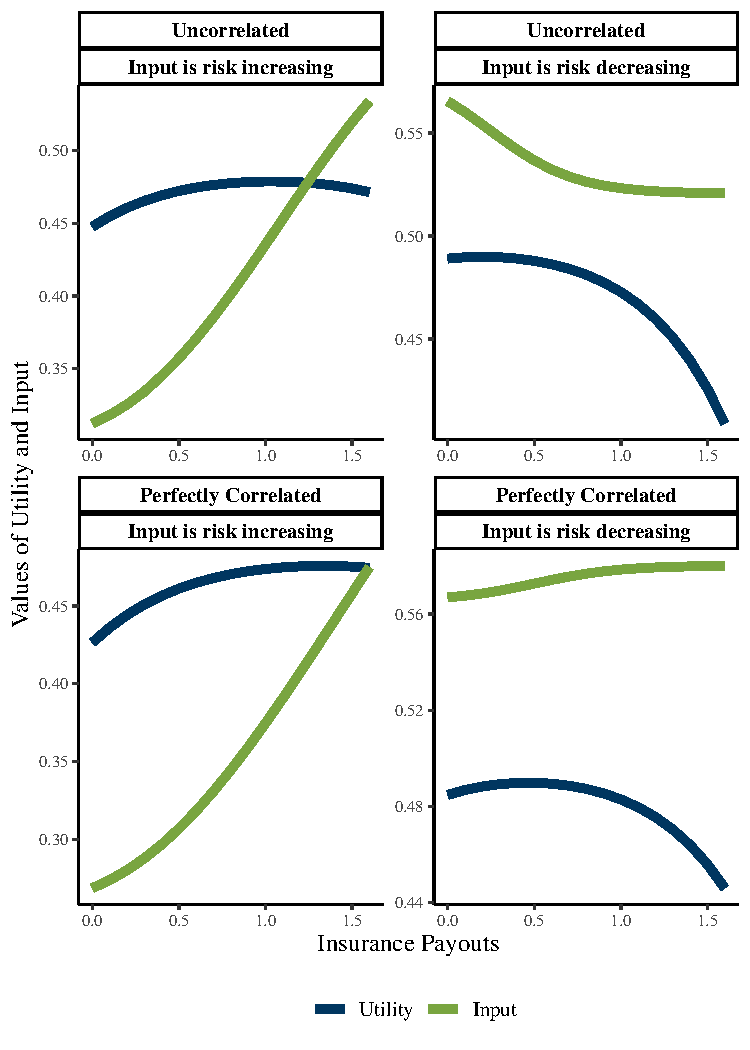
\includegraphics[keepaspectratio]{ibi-behavior_files/figure-pdf/fig-iter-1.pdf}}

}

\caption{\label{fig-iter}Utility (blue lines) and optimal input use
(green lines) with index insurance. Shocks are uncorrelated with high
mean productivity (\(\alpha=0.75\)), high risk aversion \(a=3\), and
relatively high variance in both shocks (\(\sigma_{w}=0.4\) and
\(\sigma_{t}=0.4\))}

\end{figure}%

Optimal input use changes monotonically with index insurance for both
risk increasing and decreasing inputs (Figure~\ref{fig-iter}). Fishers
use more risk increasing inputs for both contract specifications. For
risk decreasing inputs, fishers will only use less inputs if the
contract is specified on extraction risk. Otherwise, fishers will use
more risk decreasing inputs if the contract is triggered on stock risk
as shown in the bottom right panel of Figure~\ref{fig-iter}.

The concavity of utility, as demonstrated by the blue parabolas in all
panels of Figure~\ref{fig-iter}, implies there exists an optimal amount
of insurance for fishers to buy. The monotoncity of input use in all
cases suggests that the insurance level that maximizes utility will
preserve the sign of input changes. Therefore, an endogenous choice of
insurance will not affect the direction of input change, but it will
affect the magnitude.

For example, contracts protecting against stock risks have peak
parabolas further right than contracts on extraction risks in
Figure~\ref{fig-iter}. Fishers would be better off with higher levels of
insurance coverage. Allowing fishers to choose insurance coverage
ensures that the choice of insurance and input use changes are welfare
improving and will not bias input choices with over or under investment
of insurance. Simulations moving forward will allow fishers to choose
both inputs and insurance coverage.

With two choice variables,\(\gamma\) and \(x\), Equation~\ref{eq-maxsim}
becomes Equation~\ref{eq-maxsim2}:

\begin{equation}\phantomsection\label{eq-maxsim2}{
\begin{aligned}
U&\equiv\max_{x,\gamma}\mathbb{E}[u]=\mathbb{E}[(1-\exp(-a(\pi(x,\hat\beta,\theta,\omega)+\mathbb{I}(\gamma))]\\
\mathbb{I}(\gamma)&=\begin{cases}-\rho\gamma & \text{if } \omega\ge \bar\omega\\
(1-\rho)\gamma & \text{if } \omega<\bar\omega
\end{cases}
\end{aligned}
}\end{equation}

Furthermore, we run two groups of simulations: (i) one where the
insurance contract indemnifies on \(\omega\), as in
Equation~\ref{eq-maxsim}; and (ii) one where the index is constructed on
\(\theta\), to present results for both Proposition~\ref{prp-ind} and
Proposition~\ref{prp-theta}.

Contract specification and risk effects control the direction of input
change in fisheries. Insurance contracts that protect against extraction
risks lead to increases or decreases in optimal input use contingent on
the underlying risk effects of the input. All optimal choices of risk
decreasing inputs, shown as red bars in Figure~\ref{fig-corr}, decreased
if the contract was specified on extraction risks.

The productivity of inputs strongly influences the magnitude of change
in input use particularly for risk decreasing inputs. When inputs are
relatively less productive (left panel, \(\alpha=0.25\)), fishers are
more willing to reduce the unproductive input in favor of the protection
offered by insurance. They lose less in production while gaining more
variance reduction by substituting with insurance. Therefore an
important tradeoff exists for risk reducing inputs that does not exist
for risk increasing inputs. Fishers demonstrate smaller absolute changes
in input use for risk decreasing inputs than risk increasing
particularly at higher mean productivity levels in
Figure~\ref{fig-corr}. Risk increasing inputs exert stronger effects
towards overfishing than risk decreasing inputs have towards
conservation.

\begin{figure}

\centering{

\pandocbounded{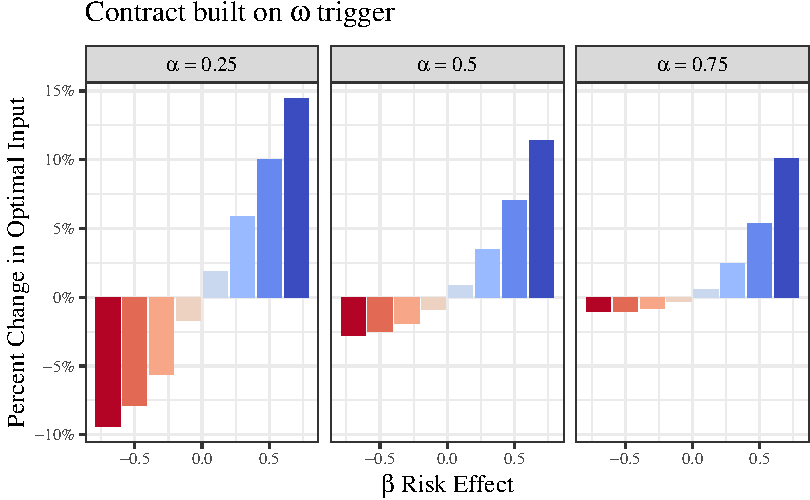
\includegraphics[keepaspectratio]{ibi-behavior_files/figure-pdf/fig-corr-1.pdf}}

}

\caption{\label{fig-corr}Percentage change in optimal input with an
index insurance contract using extraction risk, \(\omega\), as the
index. Risk increasing inputs (blue bars) always increase input use,
while risk decreasing inputs (red bars) always decrease input use. Each
panel indicates the mean productivity (\(\alpha\)) of the input.}

\end{figure}%

Contracts built on \(\theta\) as the index always lead towards
overfishing because of the inherent risk increasing characteristics of
\(f(x)\) (Figure~\ref{fig-corr-theta}). Insurance protects against risk.
Fishers are incentivized to raise risk increasing input use if protected
against the additional risk. Inputs that are more productive and more
risky with higher levels of \(\alpha\) will be used more. The right most
panel of Figure~\ref{fig-corr-theta} shows the highest effect where
input changes could reach as high as 18\%. Extraction risk in \(h(x)\)
has little influence on changes in optimal input use when the contract
is specified on stock risk. Across all levels of \(\beta\), the
magnitude of change remains relatively constant for a given productivity
level.

\begin{figure}

\centering{

\pandocbounded{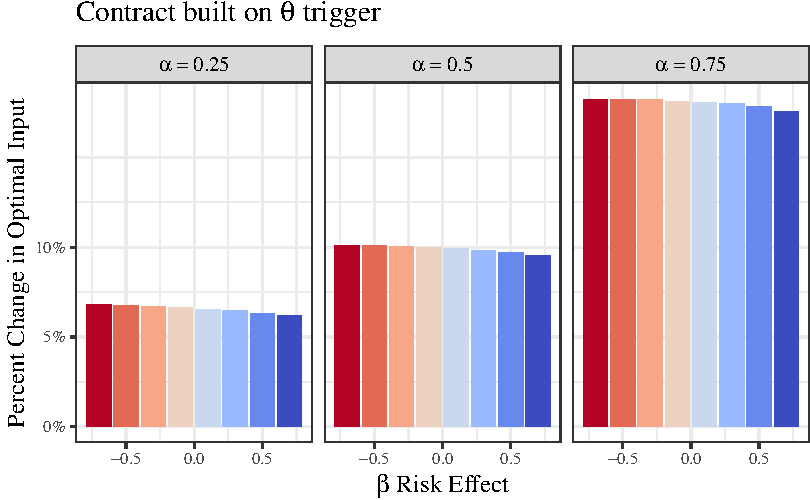
\includegraphics[keepaspectratio]{ibi-behavior_files/figure-pdf/fig-corr-theta-1.pdf}}

}

\caption{\label{fig-corr-theta}Percentage change in optimal input with
an index insurance contract using stock risk, \(\theta\), as the index.
Risk increasing inputs (blue bars) and risk decreasing inputs (red bars)
always increase input use. Each panel indicates the mean productivity
(\(\alpha\)) of the input.}

\end{figure}%

Magnitude of input changes are sensitive to other parameters beyond just
mean production elasticity (\(\alpha\)). We quickly demonstrate some
comparative statics of other important variables such as risk aversion
(Panel A in Figure~\ref{fig-sum}), trigger thresholds (Panel B),
variance of the extraction risk \(\sigma_\omega\) (Panel C), and
variance of the stock risk \(\sigma_\theta\) (Panel D). In each panel,
we show the results for the contracts specified on stock risk
(\(\theta\)) and extraction risk (\(\omega\)). The x-axis of each panel
is the extraction risk effect coefficient \(\beta\), while the y-axis is
the percent change in input use with index insurance compared to no
insurance. Different colors represent the comparative statics of each
new parameter. Across all panels, the new parameters affect only the
magnitude of change. The direction of change continues to be determined
by risk effects and contract specification.

More risk averse fishers respond more aggressively to insurance and make
relatively more changes toward their input decisions (Panel A in
Figure~\ref{fig-sum}). Risk aversion implies more sensitivity towards
risk. The protection from insurance has greater marginal value for more
risk averse fishers. Greater marginal value of insurance means they can
invest less into risk reducing inputs than before, and have more
protection from greater shocks with risk increasing inputs.

Different triggers also lead to different magnitudes of input change,
but do not affect the sign changes. While necessary for applying
Lemma~\ref{lem-mp} and Lemma~\ref{lem-theta} in the proofs, the results
of Proposition~\ref{prp-ind} and Proposition~\ref{prp-theta} would
appear to hold if \(\bar\omega\ne0\) and \(\bar\theta\ne0\). Higher
trigger levels protect against extreme or catastrophic shocks. However,
those shocks occur much less frequently than those closer to the mean.
Fishers are less incentivized to change their expected production levels
in the event of rare events. Offering different insurance contracts does
change the optimal choice of insurance in line with the results of
Lichtenberg and Iglesias (2022).

Fisher input choice is much more responsive to insurance protection from
more variable shocks (Panel C and D Figure~\ref{fig-sum}), but it
depends on the insurance contract. Similar to risk aversion, the greater
the shocks the greater the marginal value of insurance to mitigate those
shocks. In more volatile environments, insurance provides significantly
more income smoothing leading to similar incentives as the higher risk
aversion example. Shocks the insurance does not protect against has
little influence on fisher input decisions. If the insurance is designed
to protect against one specific shock, it is unsurprising changes in the
other independent shock do not affect fishers decisions.

\begin{figure}

\centering{

\pandocbounded{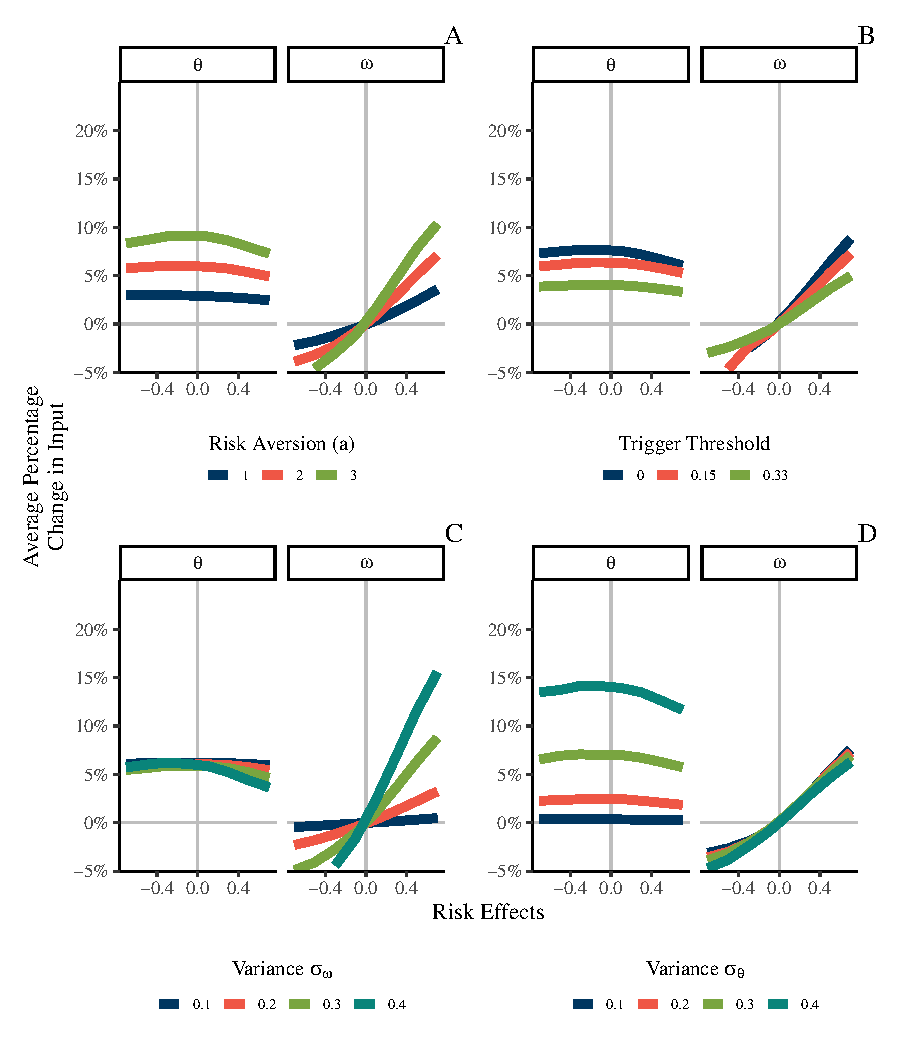
\includegraphics[keepaspectratio]{ibi-behavior_files/figure-pdf/fig-sum-1.pdf}}

}

\caption{\label{fig-sum}Risk Aversion (A), trigger threshold (B), stock
variance \(\sigma_{omega}\) (C), and extraction variance
\(\sigma_{theta}\) (D) all influence the magnitude of change in input
use. Mean production elasticity is set to 0.5. Average percent change in
input (y-axis) is summarized across all other parameter combinations for
each risk effect value of \(\beta\). Contracts built on extraction risk
are in the subpanels with \(\omega\), while contracts built on stock
risk are indicated by the \(\theta\) subpanel.}

\end{figure}%

\subsection{Application to Norwegian
Fisheries}\label{application-to-norwegian-fisheries}

Fishery extraction risk effects are rarely estimated, though appear
crucial to determining the magnitude of input change with index
insurance. The only study to date that calculates risk effects is that
of Asche \emph{et al.} (2020). They used a non-linear estimator to
calculate the production and risk parameters of a Just-Pope function
across four different vessel types. We will use their coefficient
calculations to calibrate an estimate of the magnitude of input and
harvest change that index insurance would incentivize if offered to
important Norwegian fisheries.

Asche \emph{et al.} (2020) aggregated by vessel type and not species, so
there is no reasonable estimate for biomass. They accounted for biomass
using fixed effects in their regression, but without additional
information we cannot parameterize the mean and variance of biomass.
Therefore, our simulations normalize mean biomass to 1 and we assume the
stock shocks, \(\theta\), have a normal distribution and test different
levels of variance. Norwegian fisheries are well managed so the stock
variance could be mitigated through quota systems or accurate stock
assessments. The simulation model uses three inputs: capital \(k\),
labor \(l\), and fuel \(f\), yielding the following profit in
Equation~\ref{eq-sim3}:

\begin{equation}\phantomsection\label{eq-sim3}{
\pi(k,l,f)=k^{\alpha_k}l^{\alpha_l}f^{\alpha_f}(\hat\beta+\theta)+\omega k^{\beta_k}l^{\beta_l}k^{\beta_f}-c_kk^2-c_ll^2-c_ff^2
}\end{equation}

Mean production, \(\alpha\), and risk, \(\beta\), elasticities control
the stock and extraction risk effects respectively. Each parameter is
indexed to a particular input through the subscript, e.g.~fuel mean
production elasticity is \(\alpha_f\). Fishers in the simulation choose
inputs and insurance coverage to maximize expected utility. We show
their choice based on a \(\omega\) contract
(Equation~\ref{eq-maxasche}), but also run a model specification with a
contract built on \(\theta\).

\begin{equation}\phantomsection\label{eq-maxasche}{
\begin{aligned}
U&\equiv\max_{\gamma,k,l,f}\mathbb{E}[u]=\mathbb{E}[u(k^{\alpha_k}l^{\alpha_l}f^{\alpha_f}(\hat\beta+\theta)+\omega k^{\beta_k}l^{\beta_l}k^{\beta_f}-c_kk^2-c_ll^2-c_ff^2+\mathbb{I}(\gamma)]\\
\mathbb{I}(\gamma)&=\begin{cases}-\rho\gamma & \text{if } \omega\ge \bar \omega\\
(1-\rho)\omega& \text{if } \omega<\bar \omega
\end{cases}
\end{aligned}
}\end{equation}

Table~\ref{tbl-asche} shows the production and risk elasticities of the
three vessel types found in Norway\footnote{In Asche \emph{et al.}
  (2020), they also estimate a fourth vessel type, purse seiners.
  However the point estimate for mean production elasticity for labor
  was negative which violates our assumption of increasing \(f(x)\).
  Therefore we drop purse seiners from our analysis.}.

\begin{longtable}[]{@{}
  >{\raggedright\arraybackslash}p{(\linewidth - 12\tabcolsep) * \real{0.2609}}
  >{\raggedleft\arraybackslash}p{(\linewidth - 12\tabcolsep) * \real{0.1304}}
  >{\raggedleft\arraybackslash}p{(\linewidth - 12\tabcolsep) * \real{0.1304}}
  >{\raggedleft\arraybackslash}p{(\linewidth - 12\tabcolsep) * \real{0.1304}}
  >{\raggedleft\arraybackslash}p{(\linewidth - 12\tabcolsep) * \real{0.1159}}
  >{\raggedleft\arraybackslash}p{(\linewidth - 12\tabcolsep) * \real{0.1159}}
  >{\raggedleft\arraybackslash}p{(\linewidth - 12\tabcolsep) * \real{0.1159}}@{}}

\caption{\label{tbl-asche}Production and Risk elasticities of Norwegian
Fisheries from Asche et al., (2020)}

\tabularnewline

\toprule\noalign{}
\begin{minipage}[b]{\linewidth}\raggedright
\end{minipage} & \begin{minipage}[b]{\linewidth}\raggedleft
\(\alpha_k\)
\end{minipage} & \begin{minipage}[b]{\linewidth}\raggedleft
\(\alpha_l\)
\end{minipage} & \begin{minipage}[b]{\linewidth}\raggedleft
\(\alpha_f\)
\end{minipage} & \begin{minipage}[b]{\linewidth}\raggedleft
\(\beta_k\)
\end{minipage} & \begin{minipage}[b]{\linewidth}\raggedleft
\(\beta_l\)
\end{minipage} & \begin{minipage}[b]{\linewidth}\raggedleft
\(\beta_f\)
\end{minipage} \\
\midrule\noalign{}
\endhead
\bottomrule\noalign{}
\endlastfoot
Coastal Seiners & 0.294 & 0.421 & 0.457 & 0.184 & -0.432 & 0.119 \\
Coastal Groundfish & 0.463 & 0.421 & 0.355 & 0.965 & -0.080 & 0.113 \\
Groundfish Trawlers & 0.210 & 0.106 & 0.531 & -2.788 & -0.110 &
-0.024 \\

\end{longtable}

We use the same parameter space as the previous simulations to test the
sensitivity of fisher input choices with index insurance. We plot the
distribution of input change after insurance for all combination of
parameters in Figure~\ref{fig-asche-input} based on a contract with
\(\omega\) as the index. Figure~\ref{fig-asche-input} also allow us to
examine whether the conditions of Proposition~\ref{prp-samre} hold with
real world combinations. We report the median change as an indicator of
the general direction of input change.

\begin{figure}

\centering{

\pandocbounded{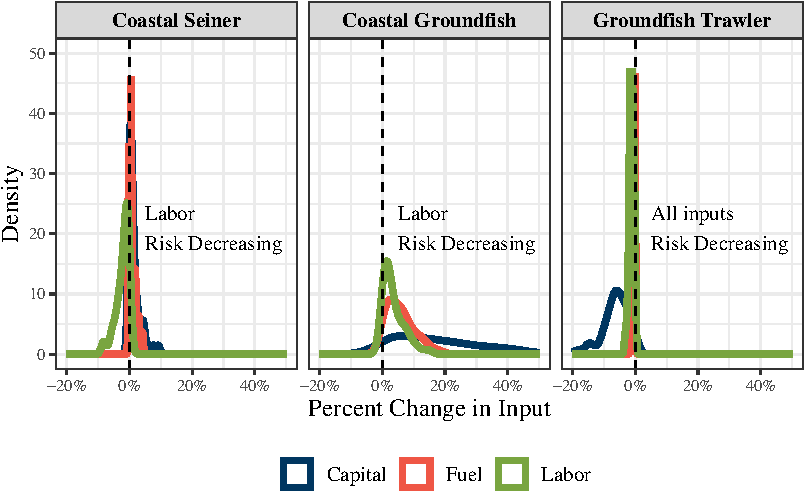
\includegraphics[keepaspectratio]{ibi-behavior_files/figure-pdf/fig-asche-input-1.pdf}}

}

\caption{\label{fig-asche-input}Density plots of the percent change in
input use for each vessel type in Norwegian fisheries with contracts
built on extraction risk \(\omega\). The dashed black line represents no
change in input use. Risk decreasing inputs are labeled.}

\end{figure}%

Most changes in inputs tend to change in the direction expected of their
own individual risk effects. For example, fuel and capital are risk
increasing inputs for Coastal Seiners and saw small, but positive
increases. Labor was risk decreasing and saw a decline in use. This
indicates that the conditions of Proposition~\ref{prp-samre} can hold.
The relative even balance between the marginal productivity elasticities
and risk elasticities perhaps determine the conditions.

Labor in the Coastal Groundfish fishery is risk decreasing, yet always
saw an increase in the simulations. The risk parameter of labor is
relatively small compared to the risk increasing coefficients of capital
and fuel. The cross partial mix of the inputs may explain why fishers
add more labor. As insurance strongly incentivizes capital and fuel
increases, labor must also increase to further enhance those other
inputs. Here, the conditions of Proposition~\ref{prp-samre} do not hold.

Every input in the groundfish trawler fishery was risk decreasing. With
contracts on extraction risks all inputs saw a decline. The largest
decline was in capital, because capital possesses the strongest risk
decreasing effect out of all inputs.

Recreating the same analysis with contracts on stock risks shows the
propensity for these types of contracts to stimulate increased input use
regardless of risk effects Figure~\ref{fig-asche-all}. It appears all
inputs saw similar increases in each fishery with the exception of
capital in the groundfish trawlers. While capital still increased, it
did so at a much smaller rate. Capital in the groundfish trawler fishery
is the most risk decreasing input out of all the fisheries. Fishers do
not need to expand capital production in this case because it already
reduces so much risk. Adding insurance marginally reduces some risk,
hence the increase, but is not needed as much compared to other
fisheries with weaker risk reducing inputs.

\begin{figure}

\centering{

\pandocbounded{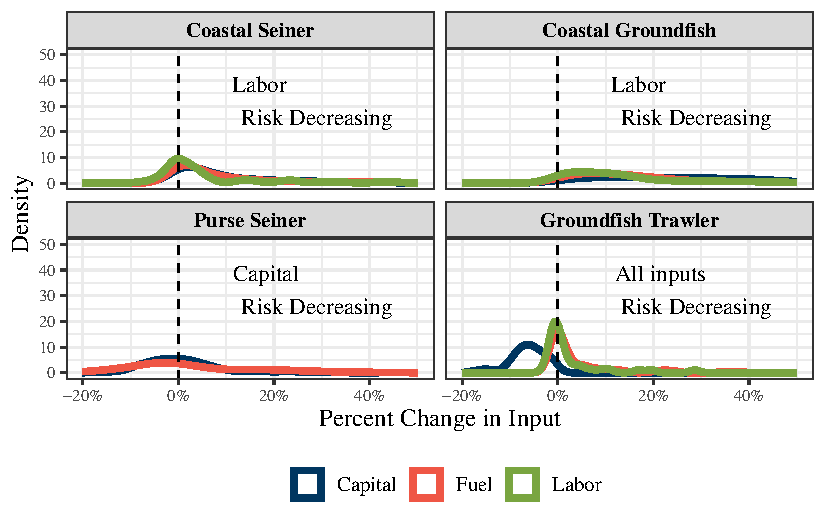
\includegraphics[keepaspectratio]{ibi-behavior_files/figure-pdf/fig-asche-all-1.pdf}}

}

\caption{\label{fig-asche-all}Density plots of the percent change in
input use for each vessel type in Norwegian fisheries with insurance
contracts built on stock risk \(\theta\). The dashed black line
represents no change in input use. Risk decreasing inputs are labeled.}

\end{figure}%

Input changes lead to harvest changes. We examine the total change in
harvest for all parameters in Figure~\ref{fig-asche} for a contract
triggered on \(\omega\). Overall, insurance leads to relatively small
changes in harvest for all fisheries, but increases are stronger than
decreases. Coastal Groundfish see the largest and most consistent
increase in harvest. Median harvest increased by 10\% with a max
increase of 36\%. Coastal Groundfish have the most risk increasing
inputs out of the estimated fisheries and always saw increases in input
use (Figure~\ref{fig-asche-input}).

\begin{figure}

\centering{

\pandocbounded{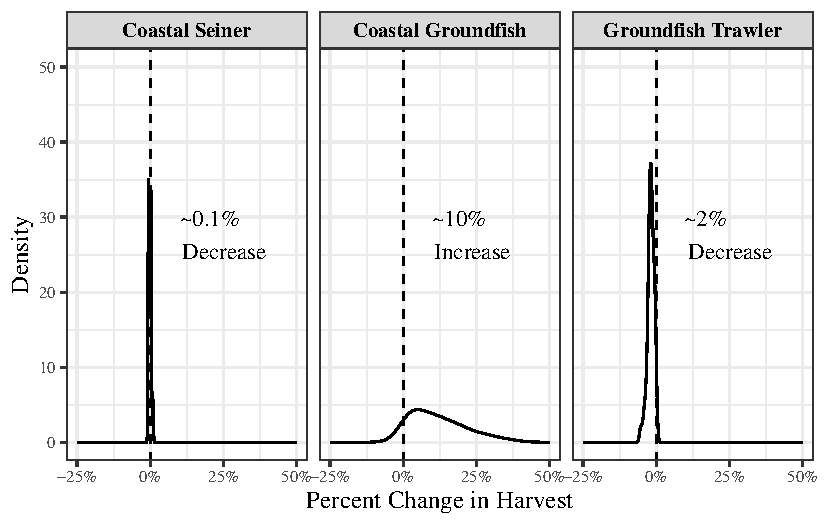
\includegraphics[keepaspectratio]{ibi-behavior_files/figure-pdf/fig-asche-1.pdf}}

}

\caption{\label{fig-asche}Density plots of the percent change in harvest
for each vessel type in Norwegian fisheries from an insurance contract
trigged on extraction risks \(\omega\). The dashed line represents no
change in harvest. The text labels represent the median percent change
in harvest for each vessel type.}

\end{figure}%

Coastal Seiners had a relatively balanced spectrum of risk effects. The
input mix in this case led to both increases and decreases in input use,
which on net led to near zero changes in harvest. There is a slight skew
towards increased harvest, but drastically less than the Coastal
Groundfish fishery.

Groundfish trawlers consistently see small decreases of 2\% in harvest
(Figure~\ref{fig-asche}). All inputs are risk decreasing with capital
having the strongest risk effect out of all inputs across all fisheries.
However, it has a relatively low marginal productivity. Insurance
decreases trawler capital use by about 8\%, but the low productivity
leads to only a 2\% decrease in overall harvest.

Applying an insurance contract indemnified on \(\theta\) instead of
\(\omega\) shifts the direction towards more overfishing
(Figure~\ref{fig-asche-theta}). Prominent shifts occur in all fleets.
For example, in Figure~\ref{fig-asche}, the percent change in harvest
for Coastal Seiners is indistinguishable from zero. With a \(\theta\)
index contract, Coastal Seiners would increase harvest by 18\%
(Figure~\ref{fig-asche-theta}).

Despite the risk decreasing dominance of capital in groundfish trawlers,
fishers will choose to increase production as insurance drastically
protects against the added harvest risk. This result most clearly shows
the impact of different insurance contracts and the potential for
maladaptive behavior change. Without considering all the margins for
change, insurance protecting against biological risk will encourage
overfishing without additional constraints.

\begin{figure}

\centering{

\pandocbounded{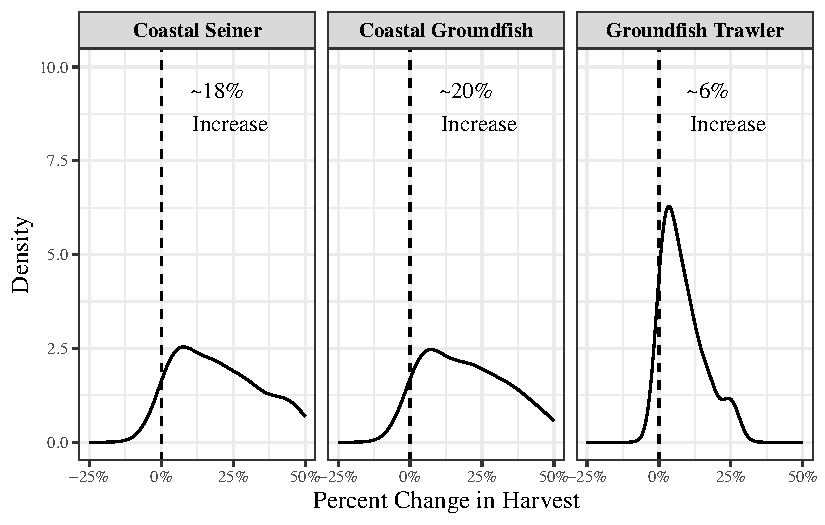
\includegraphics[keepaspectratio]{ibi-behavior_files/figure-pdf/fig-asche-theta-1.pdf}}

}

\caption{\label{fig-asche-theta}Density plots of the percent change in
harvest for each vessel type in Norwegian fisheries with insurance
contract indemnified on biological risk \(\theta\). The dashed line
represents no change in harvest. The text labels represent the median
percent change in harvest for each vessel type.}

\end{figure}%

\section{Discussion}\label{sec-disc}

This paper makes four distinct contributions. First, if fishery
production is specified to traditional fishery models, then index
insurance will inherently lead to overfishing. Second, with more
flexible specifications of risky production, fishers may increase or
decrease the use of their inputs contingent on the extraction risk
effects of their inputs when offered insurance contracts. Third,
contract specification influences fisher behavior. Contracts that use
stock risk as a trigger will always lead to increases, while contracts
that use extraction shocks could increase or decrease. Fourth, multiple
inputs may interact in unexpected ways when compared to single input
behavior.

The fundamental driver of fishers' behavior changes is whether the
marginal change in productivity is balanced by the marginal change in
risk. Fishers are more willing to increase production if insurance
negates the additional risk of expanded production. Since insurance
lowers risk, fishers need less self insurance through risk reducing
inputs and can reduce their overall input use. However, using less
inputs implies less catch and revenue creating a unique tension for risk
decreasing inputs. Across all simulations, decreased input use was
smaller than increased input use holding all other parameters constant.
This is a clear demonstration of the tradeoff fishers face when
considering risk decreasing input choices with insurance. Behavior
change in fisheries will lean towards expanding production creating a
dilemma for conservation efforts.

Index insurance would improve welfare in Norwegian fisheries, but also
lead to changes in harvest that depends on the extraction risk effects
of fishing fleets. The average utility gain was small for all
simulations at 2\% on average\footnote{The utility gains are smaller by
  construction as we manually introduce basis risk with an imperfect
  insurance contract that cannot simultaneously protect both risks.},
but always positive indicating index insurance would be welfare
improving. Therefore, insurance can provide immediate benefit to
fishers, but the policymaker must take measures to mitigate the preserve
incentive to expand fishing production. Otherwise, the long term health
of the stock could be degraded and fishers would be worse off in the
long run (Müller \emph{et al.} 2017; John \emph{et al.} 2019; Bulte and
Haagsma 2021). In the case of Norwegian fisheries, increased harvest
could reach up to 50\% with insurance contracts built on stock risk
placing additional strain on the stock.

Norwegian pelagic groundfish trawlers would have the opposite
considerations. When offered insurance they reduced their harvest by
2\%. Though small, it will lead to improved fishery sustainability. The
long term benefit of insurance would increase with improved stock
health. The decline in harvest was driven by a reduction in
overcapitalization, because capital was a significant risk decreasing
input. Policymakers should attempt to identify fisheries with risk
decreasing inputs for insurance contracts to improve sustainability if
index insurance is to operate in isolation of other policies.

Ex-ante identification of input risk effects is challenging. Extraction
risk effects remain an elusive concept in fisheries, and need to be
estimated in order to articulate more accurate behavior changes of
fishery index insurance. Crop covers and pesticide provide clear
examples of risk decreasing inputs in agriculture, but what do risk
decreasing inputs look like in fisheries? Asche \emph{et al.} (2020)
provide empirical evidence of the existence of risk decreasing inputs,
but do not elaborate on why or how labor and capital directly decrease
risk. Labor is perhaps the more intuitive risk decreasing input.
Technical expertise of crew and captains can hedge against luck when
fishing (Alvarez \emph{et al.} 2006). Better trained crew can deploy
gear in a safe and timely manner, increasing the likelihood of effective
sets.

Fuel as a risk increasing input in fisheries makes intuitive sense as
well. Fuel is used to power vessels and is a direct cost of fishing.
Fishers explore productive fishing grounds for the best location. Every
hour at sea increases the harvest reward, but also the chances of
failure.

Capital is a more complex input, because it is shown to be both risk
increasing and decreasing. Capital in fisheries typically refer to
vessel tonnage, engine power, and gear technology. Greater capital
increases risk because it allows fishers to explore more fishing
grounds, use more efficient gear, and fish in more adverse weather
conditions. Alternatively, having larger vessels may be a risk reducing
input when common pool resources incentivize the race to fish, as the
sooner a fisher harvests from the stock, they assure their income at the
expense of other fishers. Adding risk aversion to standard models of
common pool fisheries suggests fishers should lower their capital use
compared to risk neutral allocations (Mesterton-Gibbons 1993; Tilman
\emph{et al.} 2018). Yet, overcapitalization and overfishing are more
often observed in the real world. Either fishers are never risk averse
or the risk effects of capital are not as simple as the standard model
suggests. When capital is allowed to be risk decreasing, optimal capital
choices are much higher than optimal capital without risk. Thus, fishers
can still make rational, risk averse decisions even while overfishing.

Fishers exposure to multiple sources of risk further necessitates
insurance, but also makes it more challenging to design.
Proposition~\ref{prp-ind} and Proposition~\ref{prp-theta} shows the
effects of insurance contract specifications on harvest. The assumed
volatility of more fish in the ocean leads the harvest function to
implicitly be risk increasing in our specification of stochastic
production. With this assumption, designing a contract around a stock
shock will bias the results towards more overfishing. In the Norwegian
fisheries, contracts built on stock risk increased median fish harvest
in all fisheries. However, the leading candidates for possible indices
in fisheries index insurance are currently weather variables most often
associated with biological stock risks (Watson \emph{et al.} 2023).
Designing contracts solely on these variables may lead to harvest
increases that run contrary to conservation goals.

However, most bioeconomic models simplify the complex effects of stock
dynamics into multiplicative or additive forms as modeled in this paper.
Instead, different forms of risk could be embedded into the biological
component of fishery models. Stock variance could be greater in
overfished stocks instead of healthier ones, reflecting more
vulnerability in weaker states (Sims \emph{et al.} 2018). Adapting
alternative, more biologically focused specifications of stock risk
could change the behavioral effects of insurance. Fishers may be more
willing to expose themselves to greater risk at more vulnerable stock
levels with insurance. Alternatively, insurance could help mitigate risk
and incentivize fishers to move toward healthier stocks with less
variance by alleviating income pressures to fish. Further analysis is
required to understand the full implications of stock risk effects in
fisheries.

The transfer between inputs and insurance reflects the substitution
between self-insurance and formal insurance (Quaas and Baumgärtner
2008). If index insurance is designed to reduce fishing capacity,
efforts must be made to ensure that it does not take away from the self
insurance capacity of fishers. Labor appears to be consistently risk
reducing and acts as a form of self insurance. If index insurance
incentivizes captains to hire less crew, the stock of fish may be
preserved, but less employment may reverberate throughout the community.
Fishing is often a primary employment opportunity in coastal
communities. The resiliency of the community would be compromised rather
than enhanced with fewer jobs. The same idea applies to capital. If
fishers are over investing in capital to hedge against some form of
risk, policymakers need to be sure the insurance is replacing
maladaptive self insurance behavior.

The primary form of risk mitigation in fisheries is management. To this
point our analysis explicitly modeled scenarios without the existence of
management. We wanted to analyze the interaction of insurance on fisher
behavior in unconstrained settings first to derive a clearer incentive
structure. Most fisheries are managed in some form. The interaction
between management and insurance may be complementary or substitutes.
For example, well managed fisheries that have responsive harvest control
rules may not need insurance. The management system is already providing
the necessary risk protection. Insurance demand and uptake may be low in
these fisheries.

Insurance could instead complement management to provide the financial
relief that management cannot offer. Managers often focus on the
biological health of the fishery that can run at odds with fishers'
desires to enhance their income. Insurance can act as the financial
relief and allow managers to pursue more active strategies to protect
fish stocks without political resistance from lowered quotas.
Additionally, management can provide the constraints on insurance moral
hazard so the income smoothing benefits are passed to fishers, but not
the long term degradation. The interaction between insurance and
management requires further investigation especially with the numerous
management strategies that exist in fisheries.

Design and access of insurance must also consider equity. The current US
federal disaster relief program is inequitable with bias towards large
industrial vessels (Jardine \emph{et al.} 2020). Current US farm
subsidies, including insurance premiums, are heavily skewed towards
large agribusinesses (White and Hoppe 2012). Dimensions of access,
procedural, representation, and distribution must all be built into the
design of new fishery index insurance programs (Fisher \emph{et al.}
2019). For example, small scale fishers may have income constraints that
prevent them from buying the initial contract. Micro-finance options
connected to insurance have been used in agriculture to alleviate this
burden with some success (Dougherty \emph{et al.} 2021). Additionally,
who receives the payouts needs thorough consideration. Payouts solely to
vessel owners may ignore support to valuable, yet vulnerable fishery
participants. Deckhands and crew are laid off during closures. The
broader community is also affected by lost income beyond fishers on the
water. Fish processors and harbors are also affected when fishing income
is lost. If index insurance payouts are going through the entire
fishery, the most vulnerable in the event of closures must be protected
as well. Contract stipulations could mandate that only cost expenses are
covered by payouts thereby including lost wages to the crew. Agriculture
contracts often are designed to directly cover expenses (He \emph{et
al.} 2020). Labor expenses could be included in the contract to ensure
that the crew is protected as well.

Our model only directly models behavior change through moral hazards.
Index insurance could be designed to incentivize other forms of
sustainable behavior change. We define three pathways insurance can
change behavior: Moral hazards, Quid Pro Quo, and Collective Action.
Moral hazards were proven in this paper to have ambiguous impacts
controlled by the risk characteristics of fishery inputs. The incentives
of moral hazards will always exist, therefore other measures could be
taken to either limit the downside behavioral effects of insurance or
stimulate other forms of sustainable behavior.

Quid Pro Quo expands contract design to explicitly build in conservation
measures. Fishers would be required to adopt sustainable practices in
order to qualify for insurance. Quid Pro Quo is already used in
agricultural insurance in the form of Good Farm Practices. Farmers must
submit management plans to US Risk Management Agency that clearly
outline their conservation practices in order to qualify for insurance.
Working closely with management agencies, insurance companies could
design contracts that require fishers to follow fishery specific
management practices. For example, fishers may be incentivized to use
more sustainable gear types, have an observer onboard, or reduce
bycatch. A stipulation in in the COAST program is for fishers to
register their vessels with the participating countries fisheries
department (Sainsbury \emph{et al.} (2019)). This step has brought
greater data clarity to small scale Caribbean fisheries.

Further research would need to uncover the full impact of Quid Pro Quo,
but an initial hypothesis would be fishers will be willing to adopt
sustainable practices so long as the marginal gain in utility from the
insurance is greater or equal to the marginal costs of the stipulated
sustainable changes. Otherwise fishers will not want to buy the
contracts and the insurance has no binding constraints to change the
fishery.

Collective action ties insurance premiums to biological outcomes to
leverage the political economy of the fishery. Insures could reduce
premiums in fisheries that have robust management practices such as
adaptive harvest control rules, stock assessments, or marine protected
areas in the vicinity. Fishers could either pressure regulators to adopt
these actions or form industry groups to undertake the required actions.
Insurers would agree to this if triggers are connected to biological
health so that negative shocks are less frequent and thus payouts occur
less. Fishers gain from the reduced insurance premium and the increased
sustainability of harvest with rigorous management in place.

Ultimately, if index insurance is to be used in fisheries, it must be
designed with clear objectives and intentions. Index insurance can meet
objectives of income stability and risk reduction, but there has been an
implicit assumption by practitioners that index insurance will always
lead to improved sustainability. Our results directly contradict that
claim with the use of traditional models. Without considering the
behavior change of fishers when adopting insurance, the outcomes may not
be as expected. New insights derived from this paper will help guide the
efficient and sustainable implementation of fisheries index insurance.

\newpage
\appendix
\renewcommand{\thefigure}{A\arabic{figure}}
\renewcommand{\thetable}{A\arabic{table}}
\setcounter{figure}{0}
\setcounter{table}{0}

\section{Appendix}\label{appendix}

\subsection{\texorpdfstring{Proof of
Lemma~\ref{lem-mp}}{Proof of Lemma~}}\label{proof-of-lem-mp}

\textbf{Lemma 3.1} \emph{Expected marginal profit is higher in bad
states for risk decreasing inputs when contracts are built on extraction
risk} \(\omega\) and shocks are uncorrelated.

\(\frac{\mathbb{E}[\partial \pi|\omega<\bar \omega]}{\partial x}-\frac{\mathbb{E}[\partial \pi|\omega>\bar \omega]}{\partial x}>0\)
if \(h_{x}(x)<0\).

\emph{Otherwise, risk increasing inputs lead to higher expected marginal
profit in the good states.}

\(\frac{\mathbb{E}[\partial \pi|\omega<\bar \omega]}{\partial x}-\frac{\mathbb{E}[\partial \pi|\omega>\bar \omega]}{\partial x}<0\)
if \(h_{x}(x)>0\)

\begin{proof}
By the first order conditions, there exist optimal values of any
individual input \(x\) that must be chosen before the realization of the
states of the world. Therefore \(h(x^*)\), \(f(x^*)\), and \(c(x^*)\)
are equal across states. Where \(x^*\) denotes the optimal input choice.

Marginal utility in both states of the world is controlled by risk
effects and the sign of the random variables. Given \(\theta\) is
independent of \(\omega\), the expected value of
\(\mathbb{E}[\theta|\omega\lessgtr\bar\omega]=0\). The difference in
expected marginal profit across insurance states is defined as:

\begin{equation}\phantomsection\label{eq-comppi1}{
\begin{aligned}
\small
\frac{\partial \mathbb{E}[\pi|\omega<\bar\omega]}{\partial x^*_m}-\frac{\partial \mathbb{E}[\pi|\omega>\bar\omega]}{\partial x^*_m}=&\mathbb{E}[\omega h_{x^*}(x^*)|\omega<\bar\omega]+\cancel{f_{x^*}(x^*)\hat{B}}+\cancel{\mathbb{E}[\theta f_x(x^*)|\omega <\bar\omega]}-\cancel{c_{x^*_m}(x^*)} \\
&-\mathbb{E}[\omega h_{x^*}(x^*)|\omega>\bar\omega]+\cancel{f_{x^*}(x^*)\hat{B}}+\cancel{\mathbb{E}[\theta f_x(x^*)|\omega >\bar\omega]}-\cancel{c_{x^*_m}(x^*)}\\
=&\mathbb{E}[\omega h_{x^*}(x^*)|\omega<\bar\omega]-\mathbb{E}[\omega h_{x^*}(x^*)|\omega>\bar\omega]
\end{aligned}
}\end{equation}

If an input is risk decreasing then \(h_{x}(x)<0\). Then
Equation~\ref{eq-comppi1} is positive and marginal profit in the bad
state is greater than the marginal profit in the good state. Adding more
of a risk reducing input reduces the negative impact in the bad state
relative to the good state.

\[
\frac{\partial \mathbb{E}[\pi|\omega<\bar\omega]}{\partial x^*}-\frac{\partial \mathbb{E}[\pi|\omega>\bar\omega]}{\partial x^*}=\overbrace{\mathbb{E}[\omega h_{x^*}(x^*)|\omega<\bar\omega]-\mathbb{E}[\omega h_{x^*}(x^*)|\omega>\bar\omega]}^{+}
\]

Repeating the same steps for risk increasing inputs \(h_{x}(x)>0\) shows
that marginal profit in the bad state is less than marginal profit in
the good state.

\[
\frac{\partial \mathbb{E}[\pi|\omega<\bar\omega]}{\partial x^*_m}-\frac{\partial \mathbb{E}[\pi|\omega>\bar\omega]}{\partial x^*_m}=\overbrace{\mathbb{E}[\omega h_{x^*}(x^*)|\omega<\bar\omega]-\mathbb{E}[\omega h_{x^*}(x^*)|\omega>\bar\omega]}^{-}
\]

\subsection{\texorpdfstring{Proof of
Lemma~\ref{lem-theta}}{Proof of Lemma~}}\label{proof-of-lem-theta}

\textbf{Lemma 3.2} \emph{Contracts built on} \(\theta\) will always lead
to higher expected marginal profits in the good state regardless of
extraction risk effects when shocks are uncorrelated

\(\frac{\mathbb{E}[\partial \pi|\theta<\bar \theta]}{\partial x}-\frac{\mathbb{E}[\partial \pi|\theta>\bar \theta]}{\partial x}<0\)

\begin{proof}
Independent shocks lead
\(\mathbb{E}[\omega|\theta \lessgtr \bar \theta]=0\).

\begin{equation}\phantomsection\label{eq-compz}{
\begin{aligned}
\small
\frac{\partial \mathbb{E}[\pi|\theta<\bar\theta]}{\partial x^*_m}-\frac{\partial \mathbb{E}[\pi|\theta>\bar\theta]}{\partial x^*_m}=&\cancel{\mathbb{E}[\omega h_{x^*}(x^*)|\theta<\bar\theta]}+\cancel{f_{x^*}(x^*)\hat{B}}+\mathbb{E}[\theta f_x(x^*)|\theta <\bar\theta]-\cancel{c_{x^*_m}(x^*)} \\
&-\cancel{\mathbb{E}[\omega h_{x^*}(x^*)|\theta>\bar\theta]}-\cancel{f_{x^*}(x^*)\hat{B}}-\mathbb{E}[\theta f_x(x^*)|\theta >\bar\theta]+\cancel{c_{x^*_m}(x^*)}\\
=&\mathbb{E}[\theta f_x(x^*)|\theta <\bar\theta]-\mathbb{E}[\theta f_x(x^*)|\theta >\bar\theta]
\end{aligned}
}\end{equation}

The concavity of \(f(x)\) leads to \(f_x(x)>0\) always.
Equation~\ref{eq-compz} can then be signed to always be negative so that
marginal profit in the good state is always higher when insurance
contracts are triggered on \(\theta\).

\[
\frac{\partial \mathbb{E}[\pi|\theta<\bar\theta]}{\partial x^*_m}-\frac{\partial \mathbb{E}[\pi|\theta>\bar\theta]}{\partial x^*_m}=\overbrace{\mathbb{E}[\theta f_{x^*}(x^*)|\theta<\bar\theta]-\mathbb{E}[\theta f_{x^*}(x^*)|\theta>\bar\theta]}^{-}
\]
\end{proof}

\end{proof}

\subsection{\texorpdfstring{Proof of
Proposition~\ref{prp-samre}}{Proof of Proposition~}}\label{sec-samre}

\textbf{Proposition 4.1} \emph{In fisheries with two inputs, when}
\(\theta\) and \(\omega\) are uncorrelated, index insurance will change
the optimal use of a specific input in accordance to an input's own risk
effect when the following sufficient condition is true:

\(\frac{\partial U}{\partial x_a x_b}>0\) when both inputs share the
same risk effects, and
\(\frac{\partial U}{\partial x_a \partial x_b}<0\) when inputs have
opposite risk effects

\emph{Otherwise, index insurance will have ambiguous effects on optimal
input choice.}

\begin{proof}
We use the same insurance design from Section~\ref{sec-common}. Fishers
now maximize expected utility by selecting two inputs. Contracts are
built on \(\omega\), but all steps follow for \(\theta\).

\begin{equation}\phantomsection\label{eq-max2}{
\begin{aligned}
U\equiv\max_{x_a,x_b}\mathbb{E}[U]=\int^{\infty}_{-\infty}&\left[ \int^{\bar \omega}_{-\infty}j(\omega,\theta)u(\pi(X,\hat{B},\theta,\omega)+(1-J(\bar \omega))\gamma)d\omega \right.\\
&\left.+\int^{\infty}_{\bar{\omega}}j(\omega,\theta) u(\pi(X,\hat{B},
\theta,\omega)-J(\bar \omega)\gamma)d\omega\right] d\theta
\end{aligned}
}\end{equation}

Taking the first order conditions yields:

\begin{equation}\phantomsection\label{eq-foc2}{
\begin{aligned}
\frac{\partial U}{\partial x_a}=&\int^{\infty}_{-\infty}\left[ \int^{\bar \omega}_{-\infty}j(\omega,\theta)u_{x_a}(\pi(X,\hat{B},\theta,\omega)+(1-J(\bar \omega))\gamma)\frac{\partial \pi}{\partial x_a}(X,\hat{B},\theta,\omega)d\omega\right.\\
&\left.+\int^{\infty}_{\bar{\omega}}j(\omega,\theta) u_{x_a}(\pi(X,\hat{B},\theta,\omega)-J(\bar \omega)\gamma)\frac{\partial \pi}{\partial x_a}(X,\hat{B},\theta,\omega)d\omega\right] d\theta\\
&=0\\
\frac{\partial U}{\partial x_b}=&\int^{\infty}_{-\infty}\left[ \int^{\bar \omega}_{-\infty}j(\omega,\theta)u_{x_b}(\pi(X,\hat{B},\theta,\omega)+(1-J(\bar \omega))\gamma)\frac{\partial \pi}{\partial x_b}(X,\hat{B},\theta,\omega)d\omega\right.\\
&\left.+\int^{\infty}_{\bar{\omega}}j(\omega,\theta) u_{x_b}(\pi(X,\hat{B},\theta,\omega)-J(\bar \omega)\gamma)\frac{\partial \pi}{\partial x_b}(X,\hat{B},\theta,\omega)d\omega\right] d\theta\\
&=0
\end{aligned}
}\end{equation}

Assuming the first order condition is satisfied, we can use the implicit
function theorem (IFT) to look at the impact of a change in the
exogenous insurance contract. Applying IFT yields a system of equations
that determine the impact of insurance on each optimal input:

\begin{equation}\phantomsection\label{eq-ivtsol}{
\begin{aligned}
&\frac{\partial x_a}{\partial \gamma}=\frac{-1}{Det}\left[\frac{\partial U}{\partial x_b \partial x_b}\frac{\partial U}{\partial x_a \partial \gamma}-\frac{\partial U}{\partial x_a \partial x_b}\frac{\partial U}{\partial x_b \partial \gamma}\right] \\
&\frac{\partial x_b}{\partial \gamma}=\frac{-1}{Det}\left[\frac{-\partial U}{\partial x_b \partial x_a}\frac{\partial U}{\partial x_a \partial \gamma}+\frac{\partial U}{\partial x_a \partial x_a}\frac{\partial U}{\partial x_b \partial \gamma}\right]
\end{aligned}
}\end{equation}

Because the determinant (DET) will always be positive by the
second-order condition, we can focus on the interior of the brackets. If
positive, then insurance will lower use of that specific input and vice
versa. The partial derivatives in Equation~\ref{eq-ivtsol} are complex.
Their complete derivations are included in Section~\ref{sec-partial}.

Lemma~\ref{lem-mp} allows us to sign the partial equations
Equation~\ref{eq-kgam} and Equation~\ref{eq-lgam} for any risk effect on
either input. Concave utility by definition leads to \(u''<0\). For
simplicity, we will only focus on
\(\frac{\partial U}{\partial x_a\partial \gamma}\), but all applies
equally to \(\frac{\partial U}{\partial x_b\partial \gamma}\). Insurance
payouts equalize profits between different states. If insurance
completely covers all loss and \(x_a\) is risk increasing, then
\(\frac{\partial U}{\partial x_a\partial \gamma}\) is positive.

\begin{equation}\phantomsection\label{eq-kgamsol}{
\begin{aligned}
\frac{U}{\partial x_a \partial \gamma}=\int^{\infty}_{-\infty}&\overbrace{j_{\theta}(\theta)J(\bar\theta)(1-J(\bar\theta))u''(\theta,\cdot)}^{-}\\
&\left[ \int^{\bar\omega}_{-\infty}\underbrace{j_{\omega}(\omega)\frac{\partial \pi}{\partial x_a}d\omega
-\int^{\infty}_{\bar{\theta}}j_{\omega}(\omega)\frac{\partial \pi}{\partial x_a}d\omega}_{-}\right] d\theta\\
>0
\end{aligned}
}\end{equation}

Suppose both inputs are risk increasing so
\(\frac{\partial U}{\partial x_a\partial \gamma}\) and
\(\frac{\partial U}{\partial x_b\partial \gamma}\) are positive. The
only way for Equation~\ref{eq-ivtsol} to be unambiguously positive is
for \(\frac{\partial U}{\partial x_a\partial x_b}\) and
\(\frac{\partial U}{\partial x_b\partial x_a}\) to be positive.

\[
\begin{aligned}
&\frac{\partial x_a}{\partial \gamma}=\overbrace{\frac{-1}{Det}}^{-}\left[\overbrace{\overbrace{\frac{\partial U}{\partial x_b \partial x_b}}^{-}\overbrace{\frac{\partial U}{\partial x_a \partial \gamma}}^{+}\overbrace{-\frac{\partial U}{\partial x_a \partial x_b}}^{-}\overbrace{\frac{\partial U}{\partial x_b \partial \gamma}}^{+}}^{-}\right] >0\\
&\frac{\partial x_b}{\partial \gamma}=\overbrace{\frac{-1}{Det}}^{-}\left[\overbrace{\overbrace{\frac{-\partial U}{\partial x_b \partial x_a}}^{-}\overbrace{\frac{\partial U}{\partial x_a \partial \gamma}}^{+}+\overbrace{\frac{\partial U}{\partial x_a \partial x_a}}^{-}\overbrace{\frac{\partial U}{\partial x_b \partial \gamma}}^{+}}^{-}\right]>0
\end{aligned}
\]

Both risk increasing inputs will be raised with index insurance.
Repeating the same steps above with risk decreasing inputs shows both
inputs unambiguously decrease with index insurance.

Now suppose inputs have mixed risk effects. For simplicity, \(x_a\) will
be risk increasing and \(x_b\) will be risk decreasing. The results will
hold for the opposite case. By Lemma~\ref{lem-mp},
\(\frac{\partial U}{\partial x_a\partial \gamma}\) is positive, while
\(\frac{\partial U}{\partial x_b\partial \gamma}\) is negative.
Equation~\ref{eq-ivtsol} will be unambiguously positive if
\(\frac{\partial U}{\partial x_a\partial x_b}\) and
\(\frac{\partial U}{\partial x_b\partial x_a}\) are negative.

\[
\begin{aligned}
&\frac{\partial x_a}{\partial \gamma}=\overbrace{\frac{-1}{Det}}^{-}\left[\overbrace{\overbrace{\frac{\partial U}{\partial x_b\partial x_b}}^{-}\overbrace{\frac{\partial U}{\partial x_a \partial \gamma}}^{+}\overbrace{-\frac{\partial U}{\partial x_a \partial x_b}}^{+}\overbrace{\frac{\partial U}{\partial x_b\partial \gamma}}^{-}}^{-}\right] >0\\
&\frac{\partial x_b}{\partial \gamma}=\overbrace{\frac{-1}{Det}}^{-}\left[\overbrace{\overbrace{\frac{-\partial U}{\partial x_b\partial x_a}}^{+}\overbrace{\frac{\partial U}{\partial x_a \partial \gamma}}^{+}+\overbrace{\frac{\partial U}{\partial x_a \partial x_a}}^{-}\overbrace{\frac{\partial U}{\partial x_b\partial \gamma}}^{-}}^{+}\right]<0
\end{aligned}
\]

The risk increasing input will be raised with index insurance, while the
risk decreasing input will be lowered.

If these conditions do not hold, then it is impossible to determine
which additive element outweighs the other, and the insurance effects on
optimal input use will be ambiguous regardless of the underlying risk
effects of an input.
\end{proof}

\subsection{Partial derivatives}\label{sec-partial}

Partial derivatives used to sign Equation~\ref{eq-ivtsol} are shown
below. For brevity, \(\pi(X,\hat B,\omega,\theta)\) is reduced to
\(\pi\).

\begin{equation}\phantomsection\label{eq-kk}{
\begin{aligned}
\frac{\partial U}{\partial x_a \partial x_a}=\int^\infty_{-\infty}&\left[ \int^{\bar \omega}_{-\infty}j(\omega,\theta)[u''(\pi+(1-J(\bar \omega))\gamma)\frac{\partial\pi}{\partial x_a}+u'(\pi+(1-J(\bar \omega))\gamma)\frac{\partial \pi}{\partial x_a x_a}]d\omega \right. \\
&\left. +\int^\infty_{\bar \omega}j(\omega,\theta)[u''(\pi-J(\bar \omega)\gamma)\frac{\partial\pi}{\partial x_a}+u'(\pi-J(\bar \omega)\gamma)\frac{\partial \pi}{\partial x_a x_a}]d\omega\right]d\theta
\end{aligned}
}\end{equation}

\begin{equation}\phantomsection\label{eq-ll}{
\begin{aligned}
\frac{\partial U}{\partial x_b \partial x_b}=\int^\infty_{-\infty}&\left[ \int^{\bar \omega}_{-\infty}j(\omega,\theta)[u''(\pi+(1-J(\bar \omega))\gamma)\frac{\partial\pi}{\partial x_b}+u'(\pi+(1-J(\bar \omega))\gamma)\frac{\partial \pi}{\partial x_b x_b}]d\omega \right. \\
&\left.\int^\infty_{\bar \omega}j(\omega,\theta)[u''(\pi-J(\bar \omega)\gamma)\frac{\partial\pi}{\partial x_b}+u'(\pi-J(\bar \omega)\gamma)\frac{\partial \pi}{\partial x_b x_b}]d\omega\right]d\theta
\end{aligned}
}\end{equation}

\begin{equation}\phantomsection\label{eq-crossl}{
\begin{aligned}
\frac{\partial U}{\partial x_a \partial x_b}=\int^\infty_{-\infty}&\left[ \int^{\bar \omega}_{-\infty}j(\omega,\theta)[u''(\pi+(1-J(\bar \omega))\gamma)\frac{\partial\pi}{\partial x_a}\frac{\partial \pi}{\partial x_b}+u'(\pi+(1-J(\bar \omega))\gamma)\frac{\partial \pi}{\partial x_a x_b}]d\omega \right. \\
& \left.\int^\infty_{\bar \omega}j(\omega,\theta)[u''(\pi-J(\bar \omega)\gamma)\frac{\partial\pi}{\partial x_a}\frac{\partial \pi}{\partial x_b}+u'(\pi-J(\bar \omega)\gamma)\frac{\partial \pi}{\partial x_a x_b}]d\omega\right]d\theta
\end{aligned}
}\end{equation}

\begin{equation}\phantomsection\label{eq-crossk}{
\begin{aligned}
\frac{\partial U}{\partial x_b \partial x_a}=\int^\infty_{-\infty}&\left[ \int^{\bar \omega}_{-\infty}j(\omega,\theta)[u''(\pi+(1-J(\bar \omega))\gamma)\frac{\partial\pi}{\partial x_a}\frac{\partial \pi}{\partial x_b}+u'(\pi+(1-J(\bar \omega))\gamma)\frac{\partial \pi}{\partial x_b x_a}]d\omega \right. \\
& \left.\int^\infty_{\bar \omega}j(\omega,\theta)[u''(\pi-J(\bar \omega)\gamma)\frac{\partial\pi}{\partial x_a}\frac{\partial \pi}{\partial x_b}+u'(\pi-J(\bar \omega)\gamma)\frac{\partial \pi}{\partial x_b x_a}]d\omega\right]d\theta
\end{aligned}
}\end{equation}

\begin{equation}\phantomsection\label{eq-kgam}{
\begin{aligned}
\frac{\partial U}{\partial x_a \partial \gamma}=\int^\infty_{-\infty}&\left[ \int^{\bar \omega}_{-\infty}j(\omega,\theta)u''(\pi+(1-J(\bar \omega))\gamma)\frac{\partial\pi}{\partial x_a}(1-J(\bar \omega)d\omega \right. \\
& \left.\int^\infty_{\bar \omega}j(\omega,\theta)u''(\pi-J(\bar \omega)\gamma)\frac{\partial\pi}{\partial x_a}(-J(\bar \omega))d\omega\right]d\theta
\end{aligned}
}\end{equation}

\begin{equation}\phantomsection\label{eq-lgam}{
\begin{aligned}
\frac{\partial U}{\partial x_b \partial \gamma}=\int^\infty_{-\infty}&\left[ \int^{\bar \omega}_{-\infty}j(\omega,\theta)u''(\pi+(1-J(\bar \omega))\gamma)\frac{\partial\pi}{\partial x_b}(1-J(\bar \omega)d\omega \right. \\
&\left.\int^\infty_{\bar \omega}j(\omega,\theta)u''(\pi-J(\bar \omega)\gamma)\frac{\partial\pi}{\partial x_b}(-J(\bar \omega))d\omega\right]d\theta
\end{aligned}
}\end{equation}

\subsection{Correlation Proofs}\label{correlation-proofs}

\begin{lemma}[]\protect\hypertarget{lem-corr}{}\label{lem-corr}

When shocks are perfectly correlated, expected marginal profit is always
higher in the good state when an input, \(x_m\), is risk increasing and
ambiguous when \(x_m\) is risk decreasing. This hold regardless of the
chosen index.

\(\frac{\mathbb{E}[\partial \pi|\omega<\bar \omega]}{\partial x_m}-\frac{\mathbb{E}[\partial \pi|\omega>\bar \omega]}{\partial x_m}<0\)
if \(h_{x_m}(X)>0\)

And,
\(\frac{\mathbb{E}[\partial \pi|\omega<\bar \omega]}{\partial x_m}-\frac{\mathbb{E}[\partial \pi|\omega>\bar \omega]}{\partial x_m}\lessgtr 0\)
if \(h_{x_m}(X)<0\).

\end{lemma}

\begin{proof}
Perfect correlation between two random variables centered at 0 imply
that whenever one variable is negative, so too is the other. Due to
this, we focus only on \(\omega\) as the index. The proof follows
identically if replaced by an index on \(\theta\).

\begin{equation}\phantomsection\label{eq-corrmp}{
\begin{aligned}
\frac{\partial \mathbb{E}[\pi|\omega<\bar\omega]}{\partial x}-\frac{\partial \mathbb{E}[\pi|\omega>\bar\omega]}{\partial x}=\cancel{f_{x}(x)}\hat{B}+\mathbb{E}[\theta f_x(x)|\omega<\bar\omega]+\mathbb{E}[\omega h_{x}(x)|\omega<\bar\omega]-\cancel c(x)\\
-\cancel{f_{x}(x)}\hat{B}+\mathbb{E}[\theta f_x(x)|\omega>\bar\omega]+\mathbb{E}[\omega h_{x}(x)|\omega>\bar\omega]-\cancel c(x)
\end{aligned}
}\end{equation}

When \(h_x(X)>0\), Equation~\ref{eq-corrmp} is always negative. Expected
marginal profit is always higher in the good trigger state when shocks
are perfectly correlated.

When \(h_x(X)<0\), Equation~\ref{eq-corrmp} is ambiguous. The sign of
each line depends on the relative effect between \(f_x(X)\) and
\(h_x(X)\). If the risk effects term dominates then
Equation~\ref{eq-corrmp} will be positive. Without further information
it is impossible to know which effect dominates.
\end{proof}

\begin{proposition}[]\protect\hypertarget{prp-corr}{}\label{prp-corr}

For feasible index insurance contracts specified at either trigger,
\(\bar\omega=0\) or \(\bar\theta=0\), when \(\omega\) and \(\theta\) are
perfectly correlated random variables, the change in the optimal input
is ambiguous when \(h_x(x)<0\) and increases when \(h_x(x)>0\).

\end{proposition}

\begin{proof}
Perfect correlation implies \(\theta<0\) when \(\omega<0\) and
\(\theta>0\) when \(\omega>0\) since both distributions have mean zero,
\(\mathbb{E}[\theta]\equiv\mathbb{E}[\omega]=0\). The bounds of the
integral can be with respect to either trigger. For simplicity, we will
use \(\bar\omega\) as the trigger, but the proof holds with
\(\bar\theta\).

\begin{equation}\phantomsection\label{eq-per}{
\begin{aligned}
\frac{U}{\partial x \partial \gamma}=&\int^{\bar\omega}_{-\infty} \int^{\bar\omega}_{-\infty}j(\omega,\theta)u''(\pi(x,\hat{B},\theta,\omega)+(1-J(\bar\omega))\gamma)\frac{\partial \pi}{\partial x}(x,\hat{B},\theta,\omega)(1-J(\bar\omega))d\omega d\theta\\
+&\int^{\infty}_{\bar\omega}\int^{\infty}_{\bar{\omega}}j(\omega,\theta) u''(\pi(x,\hat{B},\theta,\omega)-J(\bar\omega)\gamma)\frac{\partial \pi}{\partial x}(x,\hat{B},\theta,\omega)(-J(\bar\omega))d\omega d\theta
\end{aligned}
}\end{equation}

Suppose insurance fully covers the loss between states, then utility in
the good state and bad state are equal to each other so that we can
factor out like terms in Equation~\ref{eq-per}.

\begin{equation}\phantomsection\label{eq-corrsol}{
\begin{aligned}
\frac{U}{\partial x \partial \gamma}=&u''(\cdot)J(\bar\omega)(1-J(\bar\omega))\\
&\times\left[\int^{\bar\omega}_{-\infty} \int^{\bar\omega}_{-\infty}j(\omega,\theta)\frac{\partial \pi}{\partial x}(x,\hat{B},\theta,\omega)d\omega d\theta
-\int^{\infty}_{\bar\omega}\int^{\infty}_{\bar{\omega}}j(\omega,\theta) \frac{\partial \pi}{\partial x}(x,\hat{B},\theta,\omega)d\omega d\theta\right]
\end{aligned}
}\end{equation}

By \textbf{?@lem-cor}, when \(h_x(X)<0\) the interior is ambiguous so
Equation~\ref{eq-corrsol} cannot be signed, but is unambiguously
positive when \(h_x(X)>0\).
\end{proof}

\section*{References}\label{references}
\addcontentsline{toc}{section}{References}

\phantomsection\label{refs}
\begin{CSLReferences}{1}{0}
\bibitem[\citeproctext]{ref-Alvarez2006}
Alvarez, A., Schmidt, P., Alvarez, A. and Schmidt, P. (2006)
\href{https://doi.org/10.1007/s11123-006-0002-x}{Is skill more important
than luck in explaining fish catches?} \emph{J Prod Anal} \textbf{26},
15--25.

\bibitem[\citeproctext]{ref-Asche2020}
Asche, F., Cojocaru, A.L., Pincinato, R.B.M. and Roll, K.H. (2020)
\href{https://doi.org/10.1007/s10640-019-00391-2}{Production risk in the
norwegian fisheries}. \emph{Environmental and Resource Economics}
\textbf{75}, 137--149.

\bibitem[\citeproctext]{ref-Babcock1996}
Babcock, B.A. and Hennessy, D.A. (1996)
\href{https://doi.org/10.2307/1243713}{Input demand under yield and
revenue insurance}. \emph{American Journal of Agricultural Economics}
\textbf{78}, 416--427.

\bibitem[\citeproctext]{ref-Barbeaux2020}
Barbeaux, S.J., Holsman, K. and Zador, S. (2020)
\href{https://doi.org/10.3389/fmars.2020.00703}{Marine heatwave stress
test of ecosystem-based fisheries management in the gulf of alaska
pacific cod fishery}. \emph{Frontiers in Marine Science} \textbf{7},
1--21.

\bibitem[\citeproctext]{ref-Bulte2021}
Bulte, E. and Haagsma, R. (2021)
\href{https://doi.org/10.1007/s10640-021-00545-1}{The welfare effects of
index-based livestock insurance: Livestock herding on communal lands}.
\emph{Environmental and Resource Economics} \textbf{78}, 587--613.

\bibitem[\citeproctext]{ref-Cai2016}
Cai, J. (2016) \href{https://doi.org/10.1257/pol.20130371}{The impact of
insurance provision on household production and financial decisions}.
\emph{American Economic Journal: Economic Policy} \textbf{8}, 44--88.

\bibitem[\citeproctext]{ref-Carter2017}
Carter, M., Janvry, A.D., Sadoulet, E. and Sarris, A. (2017)
\href{https://doi.org/10.1146/annurev-resource-100516-053352}{Index
insurance for developing country agriculture: A reassessment}.
\emph{Annual Review of Resource Economics} \textbf{9}, 421--438.

\bibitem[\citeproctext]{ref-Cavole2016}
Cavole, L.M., Demko, A.M., Diner, R.E., et al. (2016)
\href{https://doi.org/10.5670/oceanog.2016.32}{Biological impacts of the
2013--2015 warm-water anomaly in the northeast pacific: Winners, losers,
and the future}. \emph{Oceanography} \textbf{29}, 273--285.

\bibitem[\citeproctext]{ref-Cheung2021}
Cheung, W.W.L., Frölicher, T.L., Lam, V.W.Y., et al. (2021)
\href{https://www.science.org}{Marine high temperature extremes amplify
the impacts of climate change on fish and fisheries}.

\bibitem[\citeproctext]{ref-Claassen2017}
Claassen, R., Langpap, C. and Wu, J. (2017)
\href{https://doi.org/10.1093/AJAE/AAW075}{Impacts of federal crop
insurance on land use and environmental quality}. \emph{American Journal
of Agricultural Economics} \textbf{99}, 592--613.

\bibitem[\citeproctext]{ref-Collier2009}
Collier, B., Skees, J. and Barnett, B. (2009)
\href{https://doi.org/10.1057/gpp.2009.11}{Weather index insurance and
climate change: Opportunities and challenges in lower income countries}.
\emph{Geneva Papers on Risk and Insurance: Issues and Practice}
\textbf{34}, 401--424.

\bibitem[\citeproctext]{ref-Deryugina2017}
Deryugina, T. and Konar, M. (2017)
\href{https://doi.org/10.1016/j.advwatres.2017.03.013}{Impacts of crop
insurance on water withdrawals for irrigation}. \emph{Advances in Water
Resources} \textbf{110}, 437--444.

\bibitem[\citeproctext]{ref-Dougherty2021}
Dougherty, J.P., Gallenstein, R.A. and Mishra, K. (2021)
\href{https://doi.org/10.1093/jafeco/ejab003}{Impact of index insurance
on moral hazard in the agricultural credit market: Theory and evidence
from ghana}. \emph{Journal of African Economies} \textbf{00}, 1--31.

\bibitem[\citeproctext]{ref-Eggert2004}
Eggert, H. and Tveteras, R. (2004) Stochastic production and
heterogeneous risk preferences: Commercial fishers' gear choices.
199--212 pp.

\bibitem[\citeproctext]{ref-Elabed2016}
Elabed, G. and Carter, M. (2018) Ex-ante impacts of agricultural
insurance: Evidence from a field experiment in mali.

\bibitem[\citeproctext]{ref-fao2020}
FAO (2020) \href{https://doi.org/10.4060/ca9229en}{The state of world
fisheries and aquaculture 2020. Sustinability in action}. American Oil
Chemists Society.

\bibitem[\citeproctext]{ref-fao2022}
FAO (2022) World review of capture fisheries and aquaculture insurance
2022. FAO.

\bibitem[\citeproctext]{ref-Fisher2019}
Fisher, E., Hellin, J., Greatrex, H. and Jensen, N. (2019)
\href{https://doi.org/10.1111/dpr.12387}{Index insurance and climate
risk management: Addressing social equity}. \emph{Development Policy
Review} \textbf{37}, 581--602.

\bibitem[\citeproctext]{ref-Goodwin2004}
Goodwin, B.K., Vandeveer, M.L. and Deal, J.L. (2004) An empirical
analysis of acreage effects of participation in the federal crop
insurance program. \emph{American Journal of Agricultural Economics}
\textbf{86}, 1058--1077.

\bibitem[\citeproctext]{ref-He2020}
He, J., Zheng, X., Rejesus, R. and Yorobe, J. (2020)
\href{https://doi.org/10.1111/AGEC.12558}{Input use under
cost-of-production crop insurance: Theory and evidence}.
\emph{Agricultural Economics (United Kingdom)} \textbf{51}, 343--357.

\bibitem[\citeproctext]{ref-Heck2021}
Heck, N., Beck, M.W. and Reguero, B. (2021)
\href{https://doi.org/10.1016/j.marpol.2021.104698}{Storm risk and
marine fisheries: A global assessment}. \emph{Marine Policy}
\textbf{132}, 104698.

\bibitem[\citeproctext]{ref-Herrmann2004}
Herrmann, M., Greenberg, J., Hamel, C. and Geier, H. (2004)
\href{https://doi.org/10.1577/M02-086.1}{Extending federal crop
insurance programs to commercial fisheries: The case of bristol bay,
alaska, sockeye salmon}. 352--366 pp.

\bibitem[\citeproctext]{ref-Hobday2025}
Hobday, A.J., Little, L.R., Watson, J.R. and Spillman, C.M. (2025)
\href{https://doi.org/10.1007/s11160-025-09920-3}{Parametric insurance
for climate adaptation in fisheries and aquaculture}. \emph{Reviews in
Fish Biology and Fisheries} \textbf{35}, 175--185.

\bibitem[\citeproctext]{ref-Holland2008}
Holland, D.S. (2008)
\href{https://doi.org/10.1086/mre.23.3.42629621}{Are fishermen rational?
A fishing expedition}. \emph{Marine Resource Economics} \textbf{23},
325--344.

\bibitem[\citeproctext]{ref-horowitz1993}
Horowitz, J. and Lichtenberg, E. (1993) Insurance, moral hazard, and
chemical use in agriculture. \emph{American Journal of Agricultral
Economics} \textbf{75}, 926--935.

\bibitem[\citeproctext]{ref-Jardine2020}
Jardine, S.L., Fisher, M.C., Moore, S.K. and Samhouri, J.F. (2020)
\href{https://doi.org/10.1016/j.ecolecon.2020.106691}{Inequality in the
economic impacts from climate shocks in fisheries: The case of harmful
algal blooms}. \emph{Ecological Economics} \textbf{176}.

\bibitem[\citeproctext]{ref-John2019}
John, F., Toth, R., Frank, K., Groeneveld, J. and Müller, B. (2019)
\href{https://doi.org/10.1016/J.ECOLECON.2018.11.021}{Ecological
vulnerability through insurance? Potential unintended consequences of
livestock drought insurance}. \emph{Ecological Economics} \textbf{157},
357--368.

\bibitem[\citeproctext]{ref-Just1978}
Just, R.E. and Pope, R.D. (1978)
\href{https://doi.org/10.1016/0304-4076(78)90006-4}{Stochastic
specification of production functions and economic implications}.
\emph{Journal of Econometrics} \textbf{7}, 67--86.

\bibitem[\citeproctext]{ref-Kasperski2013}
Kasperski, S. and Holland, D.S. (2013)
\href{https://doi.org/10.1073/pnas.1212278110}{Income diversification
and risk for fishermen}. \emph{Proceedings of the National Academy of
Sciences of the United States of America} \textbf{110}, 2076--2081.

\bibitem[\citeproctext]{ref-Kirkley1998}
Kirkley, J. and Strand, I.E. (1998) Characterizing managerial skill and
technical efficiency in a fishery. 145--160 pp.

\bibitem[\citeproctext]{ref-Kompas2004}
Kompas, T., Che, T.N. and Grafton, R.Q. (2004)
\href{https://doi.org/10.1080/0003684042000218561}{Technical efficiency
effects of input controls: Evidence from australia's banana prawn
fishery}. \emph{Applied Economics} \textbf{36}, 1631--1641.

\bibitem[\citeproctext]{ref-Lichtenberg2022}
Lichtenberg, E. and Iglesias, E. (2022)
\href{https://doi.org/10.1016/j.jdeveco.2022.102883}{Index insurance and
basis risk: A reconsideration}. \emph{Journal of Development Economics}
\textbf{158}.

\bibitem[\citeproctext]{ref-Mahul2001}
Mahul, O. (2001) \href{https://doi.org/10.1111/0002-9092.00180}{Optimal
insurance against climatic experience}. \emph{American Journal of
Agricultural Economics} \textbf{83}, 593--604.

\bibitem[\citeproctext]{ref-Maltby2023}
Maltby, K.M., Acosta, L., Townhill, B., Touza, J., White, P. and Mangi,
S.C. (2023) \href{https://doi.org/10.1093/icesjms/fsac003}{Exploring
fishers' perceptions of index insurance and coral reef health in the
context of climate-driven changes in extreme events}. \emph{ICES Journal
of Marine Science} \textbf{80}, 2210--2221.

\bibitem[\citeproctext]{ref-gibbons1993}
Mesterton-Gibbons, M. (1993)
\href{https://doi.org/10.1111/j.1939-7445.1993.tb00143.x}{Game-theoretic
resource modeling}. \emph{Natural Resource Modeling} \textbf{7},
93--147.

\bibitem[\citeproctext]{ref-Mishra2005}
Mishra, A.K., Nimon, R.W. and El-Osta, H.S. (2005)
\href{https://doi.org/10.1016/j.jenvman.2004.08.003}{Is moral hazard
good for the environment? Revenue insurance and chemical input use}.
\emph{Journal of Environmental Management} \textbf{74}, 11--20.

\bibitem[\citeproctext]{ref-muller2017}
Müller, B., Johnson, L. and Kreuer, D. (2017)
\href{https://doi.org/10.1016/j.gloenvcha.2017.06.010}{Maladaptive
outcomes of climate insurance in agriculture}. \emph{Global
Environmental Change} \textbf{46}, 23--33.

\bibitem[\citeproctext]{ref-muller2011}
Müller, B., Quaas, M.F., Frank, K. and Baumgärtner, S. (2011)
\href{https://doi.org/10.1016/j.ecolecon.2011.06.011}{Pitfalls and
potential of institutional change: Rain-index insurance and the
sustainability of rangeland management}. \emph{Ecological Economics}
\textbf{70}, 2137--2144.

\bibitem[\citeproctext]{ref-Mumford2009}
Mumford, J.D., Leach, A.W., Levontin, P. and Kell, L.T. (2009)
\href{https://doi.org/10.1093/icesjms/fsp100}{Insurance mechanisms to
mediate economic risks in marine fisheries}. \emph{ICES Journal of
Marine Science} \textbf{66}, 950--959.

\bibitem[\citeproctext]{ref-Murkowski2022}
Murkowski, L. (2022) Working waterfronts framework: A plan to grow and
support alaska's coastal and river communities. United States Senate.

\bibitem[\citeproctext]{ref-Oken2021}
Oken, K.L., Holland, D.S. and Punt, A.E. (2021)
\href{https://doi.org/10.1002/eap.2307}{The effects of population
synchrony, life history, and access constraints on benefits from fishing
portfolios}. \emph{Ecological Applications} \textbf{0}, 1--16.

\bibitem[\citeproctext]{ref-Outreville2014}
Outreville, J.F. (2014) Risk aversion, risk behavior, and demand for
insurance: A survey. 158--186 pp.

\bibitem[\citeproctext]{ref-Pandori2019}
Pandori, L.L.M. and Sorte, C.J.B. (2019)
\href{https://doi.org/10.1111/oik.05886}{The weakest link: Sensitivity
to climate extremes across life stages of marine invertebrates}.
\emph{Oikos} \textbf{128}, 621--629.

\bibitem[\citeproctext]{ref-Pfeiffer2020}
Pfeiffer, L. (2020) \href{https://doi.org/10.1093/icesjms/fsaa145}{How
storms affect fishers' decisions about going to sea}. \emph{ICES Journal
of Marine Science} \textbf{77}, 2753--2762.

\bibitem[\citeproctext]{ref-Pfeiffer2022}
Pfeiffer, L., Petesch, T. and Vasan, T. (2022)
\href{https://doi.org/10.1086/716856}{A safer catch? The role of
fisheries management in fishing safety}. \emph{Marine Resource
Economics} \textbf{37}, 1--33.

\bibitem[\citeproctext]{ref-Quaas2008}
Quaas, M.F. and Baumgärtner, S. (2008)
\href{https://doi.org/10.1016/j.ecolecon.2007.07.004}{Natural vs.
Financial insurance in the management of public-good ecosystems}.
\emph{Ecological Economics} \textbf{65}, 397--406.

\bibitem[\citeproctext]{ref-Ramaswami1993}
Ramaswami, B. (1993) Supply response to agricultural insurance: Risk
reduction and moral hazard effects. \emph{American Journal of
Agricultural Economics} \textbf{75}, 914--925.

\bibitem[\citeproctext]{ref-RARE2021}
RARE (2021)
\href{https://rare.org/stories-articles/insuring-the-ensurers-rares-fish-forever-program-protects-the-fishers-who-feed-the-world/}{Insuring
the ensurers: A new insurance project protects the fishers who feed the
world}.

\bibitem[\citeproctext]{ref-rogers2019}
Rogers, L.A., Griffin, R., Young, T., Fuller, E., Martin, K.S. and
Pinsky, M.L. (2019)
\href{https://doi.org/10.1038/s41558-019-0503-z}{Shifting habitats
expose fishing communities to risk under climate change}. \emph{Nature
Climate Change} \textbf{9}, 512--516.

\bibitem[\citeproctext]{ref-Sainsbury2019}
Sainsbury, N.C., Turner, R.A., Townhill, B.L., Mangi, S.C. and Pinnegar,
J.K. (2019) \href{https://doi.org/10.1038/s41558-019-0645-z}{The
challenges of extending climate risk insurance to fisheries}.
\emph{Nature Climate Change} \textbf{9}, 896--897.

\bibitem[\citeproctext]{ref-Sethi2010}
Sethi, S.A. (2010)
\href{https://doi.org/10.1111/j.1467-2979.2010.00363.x}{Risk management
for fisheries}. \emph{Fish and Fisheries} \textbf{11}, 341--365.

\bibitem[\citeproctext]{ref-Sibiko2020}
Sibiko, K.W. and Qaim, M. (2020)
\href{https://doi.org/10.1007/s12571-019-00987-y}{Weather index
insurance, agricultural input use, and crop productivity in kenya}.
\emph{Food Security} \textbf{12}, 151--167.

\bibitem[\citeproctext]{ref-Sims2018}
Sims, C., Horan, R.D. and Meadows, B. (2018)
\href{https://doi.org/10.1111/NRM.12191}{Come on feel the noise:
Ecological foundations in stochastic bioeconomic models}. \emph{Natural
Resource Modeling} \textbf{31}.

\bibitem[\citeproctext]{ref-Sloggy2025}
Sloggy, M.R., Hrozencik, R.A., Manning, D.T., Goemans, C.G. and
Claassen, R.L. (2025)
\href{https://doi.org/10.1016/j.jeem.2025.103125}{Insurance and
extraction incentives in a common pool resource: Evidence from
groundwater use in the high plains}. \emph{Journal of Environmental
Economics and Management} \textbf{130}.

\bibitem[\citeproctext]{ref-Smith2023}
Smith, K.E., Burrows, M.T., Hobday, A.J., et al. (2023)
\href{https://doi.org/10.1146/annurev-marine-032122-121437}{Biological
impacts of marine heatwaves}. \emph{Annual Review of Marine Science}
\textbf{15}, 1--27.

\bibitem[\citeproctext]{ref-Smith2005}
Smith, M.D. and Wilen, J.E. (2005) Heterogeneous and correlated risk
preferences in commercial fishermen: The perfect storm dilemma. 1--53
pp.

\bibitem[\citeproctext]{ref-Smith1996}
Smith, V.H. and Goodwin, B.K. (1996)
\href{https://doi.org/10.2307/1243714}{Crop insurance, moral hazard, and
agricultural chemical use}. \emph{The Economics of Agri-Environmental
Policy} \textbf{2}, 169--179.

\bibitem[\citeproctext]{ref-stoeffler2022}
Stoeffler, Q., Carter, M., Guirkinger, C. and Gelade, W. (2022)
\href{https://doi.org/10.1093/wber}{The spillover impact of index
insurance on agricultural investment by cotton farmers in burkina faso}.
\emph{The World Bank Economic Review} \textbf{36}, 114--140.

\bibitem[\citeproctext]{ref-sumalia2020}
Sumaila, U.R., Walsh, M., Hoareau, K., et al. (2020)
\href{https://www.oceanpanel.org/blue-}{Ocean finance: Financing the
transition to a sustainable ocean economy}. World Resources Institute.

\bibitem[\citeproctext]{ref-Tilman2018}
Tilman, A.R., Levin, S. and Watson, J.R. (2018)
\href{https://doi.org/10.1016/j.jtbi.2018.06.003}{Revenue-sharing clubs
provide economic insurance and incentives for sustainability in
common-pool resource systems keywords: Risk insurance social-ecological
systems fisheries management sustainability complex adaptive systems
agent-based model common-poo}. \emph{Journal of Theoretical Biology}
\textbf{454}, 205--214.

\bibitem[\citeproctext]{ref-Wabnitz2019}
Wabnitz, C.C.C. and Blasiak, R. (2019)
\href{https://doi.org/10.1016/j.marpol.2019.103526}{The rapidly changing
world of ocean finance}. \emph{Marine Policy} \textbf{107}, 103526.

\bibitem[\citeproctext]{ref-Watson2023}
Watson, J.R., Spillman, C.M., Little, L.R., Hobday, A.J. and Levin, P.S.
(2023) \href{https://doi.org/10.1093/icesjms/fsad175}{Enhancing the
resilience of blue foods to climate shocks using insurance}. \emph{ICES
Journal of Marine Science} \textbf{80}, 2457--2469.

\bibitem[\citeproctext]{ref-White2012}
White, T.K. and Hoppe, R.A. (2012)
\href{https://www.ers.usda.gov}{Changing farm structure and the
distribution of farm payments and federal crop insurance}.

\bibitem[\citeproctext]{ref-Wu2020}
Wu, S., Goodwin, B.K. and Coble, K. (2020)
\href{https://doi.org/10.1111/agec.12545}{Moral hazard and subsidized
crop insurance}. \emph{Agricultural Economics (United Kingdom)}
\textbf{51}, 131--142.

\end{CSLReferences}




\end{document}
